% Deactivate/Activate pause
% \documentclass[handout]{beamer}
\documentclass{beamer}

\usetheme{metropolis}
\usepackage[ruled, lined, linesnumbered, commentsnumbered]{algorithm2e}
\usepackage{fourier}
\usepackage{amssymb}
\usepackage{pifont}% http://ctan.org/pkg/pifont

\newcommand{\cmark}{\ding{51}}%
\newcommand{\xmark}{\ding{55}}%\usepackage{amsmath}

\setbeamerfont{bibliography item}{size=\scriptsize}
\setbeamerfont{bibliography entry author}{size=\scriptsize}
\setbeamerfont{bibliography entry title}{size=\scriptsize}
\setbeamerfont{bibliography entry location}{size=\scriptsize}
\setbeamerfont{bibliography entry note}{size=\scriptsize}

\usepackage{tikz,balance,multicol,multirow}
% for hdashline
\usepackage{arydshln}


\usetikzlibrary{calc, shapes, backgrounds, positioning, arrows, decorations, fit}
\usepackage{pgfplots}
\newcommand{\av}{\mathbf{a}}
\newcommand{\cv}{\mathbf{c}}
\newcommand{\dv}{\mathbf{d}}
\newcommand{\ev}{\mathbf{e}}
\newcommand{\fv}{\mathbf{f}}
\newcommand{\rv}{\mathbf{r}}
\newcommand{\sv}{\mathbf{s}}
\newcommand{\tv}{\mathbf{t}}
\newcommand{\uv}{\mathbf{u}}
% \renewcommand{\vv}{\mathbf{v}}
\newcommand{\wv}{\mathbf{w}}
\newcommand{\xv}{\mathbf{x}}
\newcommand{\yv}{\mathbf{y}}
\newcommand{\zv}{\mathbf{z}}
\renewcommand{\AA}{\mathbf{A}}
\newcommand{\BB}{\mathbf{B}}
\newcommand{\CC}{\mathbf{C}}
\newcommand{\FF}{\mathbf{F}}
\newcommand{\GG}{\mathbf{G}}
\newcommand{\RR}{\mathbf{R}}
\newcommand{\Sb}{\mathbf{S}}
%\renewcommand{\SS}{\mathbf{S}}
\newcommand{\TT}{\mathbf{T}}
\newcommand{\UU}{\mathbf{U}}
\newcommand{\VV}{\mathbf{V}}
\newcommand{\WW}{\mathbf{W}}
\newcommand{\XX}{\mathbf{X}}
\newcommand{\ZZ}{\mathbf{Z}}
\newcommand{\II}{\mathbf{I}}

\newcommand{\SD}{\mathsf{SD}}
\newcommand{\DI}{\mathsf{DI}}
\newcommand{\TM}{\mathsf{TM}}
\newcommand{\mife}{{\mathsf {miFE}}}
\newcommand{\MIFE}{\mife}
\newcommand{\disfe}{\mathsf{DiFE}}%\newcommand{\tmmife}{{\mathsf{TM\mbox{-}miFE}}}
\newcommand{\sfe}{\mathsf{1FE}}
\newcommand{\Sym}{{\sf Sym}}
\newcommand{\val}{{\sf val}}
\newcommand{\tmmife}{{\mathsf{kTMFE}}}
\newcommand{\FELin}{\mathsf{LinFE}}
\newcommand{\FEPoly}{\mathsf{PolyFE}}
\newcommand{\PolyFE}{\FEPoly}
\newcommand{\NFELin}{\mathsf{NLinFE}}
\newcommand{\FEQuad}{\mathsf{QuadFE}}
\newcommand{\sfU}{\mathsf{U}} %Universal TM
\newcommand{\sfenc}{\mathsf{enc}}
\newcommand{\fxdmife}{\mathsf{(n\!+\!1)\text{-}TMFE}}


%%% For branching program %%%%
\newcommand{\BP}{\mathsf{BP}}
\newcommand{\var}{\mathsf{var}}
\newcommand{\ToDFA}{\mathsf{ToDFA}}
\newcommand{\encinp}{\mathsf{\encode}}
\newcommand{\ed}{\mathsf{ed}} % \end already defined
%%% For random variables %%%%

\def \rd {\mathfrak{d}}
\def \rF {\mathfrak{F}}
\def \rD {\mathfrak{D}}
\def \rU {\mathfrak{U}}
\def \rc {\mathfrak{c}}
\def \rgamma {\mathfrak{\gamma}}
\def \rmu {\mathfrak{\mu}}

%%% For adversaries and games %%%
\newcommand{\aA}{\mathsf{A}}
\newcommand{\aB}{\mathsf{B}}
\newcommand{\game}{\mathbf{Game}}
\newcommand{\Event}{\mathsf{E}}
\newcommand{\aP}{\mathsf{P}}
\newcommand{\aV}{\mathsf{V}}
\newcommand{\aR}{\mathsf{R}}
\newcommand{\redunderline}[1]{\textcolor{red}{\underline{\textcolor{black}{#1}}}}

\newcommand{\ul}[1]{\ensuremath{\underline{#1}}}

%%% For product vectors and matrices %%%

\def\cA{{\mathcal A}}
\def\cB{{\mathcal B}}
\def\cC{{\mathcal C}}
\def\cD{{\mathcal D}}
\def\cE{{\mathcal E}}
\def\cF{{\mathcal F}}
\def\cG{{\mathcal G}}
\def\cH{{\mathcal H}}
\def\cI{{\mathcal I}}
\def\cJ{{\mathcal J}}
\def\cK{{\mathcal K}}
\def\cL{{\mathcal L}}
\def\cM{{\mathcal M}}
\def\cN{{\mathcal N}}
\def\cO{{\mathcal O}}
\def\cP{{\mathcal P}}
\def\cQ{{\mathcal Q}}
\def\cR{{\mathcal R}}
\def\cS{{\mathcal S}}
\def\cT{{\mathcal T}}
\def\cU{{\mathcal U}}
\def\cV{{\mathcal V}}
\def\cW{{\mathcal W}}
\def\cX{{\mathcal X}}
\def\cY{{\mathcal Y}}
\def\cZ{{\mathcal Z}}
\def\bK{\mathbf {K}}
\def\cfam{\mathcal{F}}
\def\dfam{\mathcal{M}}
\def\N{\mathbb{N}}
\def\fA{\mathbf{A}}
\def\one{\mathbbm{1}}
\newcommand{\fename}{\mathsf{FE}}
\newcommand{\iO}{\mathsf{iO}}
\newcommand{\SKE}{\mathsf{SKE}}
%------------------------------
%\newcommand{\secp}{\kappa}
%Changed on 4.9.17
\newcommand{\secp}{\lambda}
%------------------------------
\newcommand{\secparam}{\secp}
\newcommand{\noise}{\chi}
\newcommand{\noiseone}{\chi_{\alpha_1}}
\newcommand{\noisetwo}{\chi_{\alpha_2}}
\newcommand{\noisei}{\chi_{\alpha_i}}
\newcommand{\noised}{\chi_{\alpha_d}}

\newcommand{\noiseonet}{\chi_{\tilde\alpha_1}}
\newcommand{\noisetwot}{\chi_{\tilde\alpha_2}}
\newcommand{\noiseit}{\chi_{\tilde\alpha_i}}
\newcommand{\noisedt}{\chi_{\tilde\alpha_d}}

\newcommand{\noiset}{\chi_{\tilde \alpha}}
\newcommand{\noiseal}{\chi_\alpha}

% %\newif\iflncs
% %	\lncstrue
% % comment out above line to get full version

% \newif\ifext
% %   \exttrue
% % uncomment the above line to get the "extended" version with
% % conjunctions of inner products and more...

% %\iflncs
% %\usepackage{breakcites}
% %\else
% %
% 	%\usepackage[hmargin=1in,vmargin=1.25in]{geometry}
% %	\usepackage{amsthm}
%   % \usepackage{xcolor}
% 	%\usepackage[pdfstartview=FitH,colorlinks,linkcolor=blue,citecolor=blue]{hyperref}

% %\fi

% 	%\usepackage[affil-it]{authblk}
% 	%\usepackage[hmargin=0.8in,vmargin=0.8in]{geometry}
% 	%\usepackage [margin=1 in]{geometry}
% 	%\usepackage{amsthm}
	
% % 	\documentclass[orivec, envcountsame, envcountsect]{llncs}
%      \usepackage{breakcites}
% %	\usepackage{enumlist}
%     \usepackage{xcolor}
% %	\usepackage[pdfstartview=FitH,colorlinks,linkcolor=blue,citecolor=blue]{hyperref}
% %	\usepackage{fullpage}
% 	\usepackage{tabu}
% 	\newcommand\hmmax{0}
% 	\newcommand\bmmax{0}
% 	\usepackage{caption}
% 	\DeclareCaptionLabelSeparator{lsep}{ }
% 	\captionsetup{labelsep=lsep}

%\usepackage{amsfonts, amsthm, amsmath, amssymb}
%\usepackage{fullpage,caption,subcaption,enumitem,array}
%\usepackage[T1]{fontenc}
%\usepackage[latin9]{inputenc}
%\usepackage{enumitem}
\usepackage{tikz,balance}
\usetikzlibrary{calc, shapes, backgrounds, positioning, arrows, decorations, fit}
\usepackage{microtype}
\usepackage{amsmath,amsfonts,mathrsfs}
%\usepackage{amssymb}
\usepackage{url}
\usepackage{xspace,paralist}
\usepackage{nicefrac}
\usepackage{algorithmicx}
\usepackage{framed}
\usepackage{graphicx}
\usepackage{breakcites}
\usepackage{mathtools}
\numberwithin{equation}{section}
\usepackage{xcolor}
\usepackage{caption} 
\captionsetup[table]{skip=5pt}
%\usepackage{placeins}
\usepackage[]{algorithm2e}

%\pagenumbering{gobble}

% THEOREMS %%%%%%%%%%%%%%%%%%%%%%%%%%%%%%%%%%%%%%%%%%%%%%%%%%%%%%%%%%%%%%%%%%%
%
%\iflncs
%\spnewtheorem{defn}[theorem]{Definition}{\bfseries}{\rmfamily}
%\spnewtheorem{rem}[theorem]{Remark}{\bfseries}{\rmfamily}
%\else

% % Theorem definitions
% \theoremstyle{plain}
 %\newtheorem{theorem}{Theorem}[section]
% \newtheorem{lemma}[theorem]{Lemma}
% \newtheorem{proposition}[theorem]{Proposition}
% \newtheorem{corollary}[theorem]{Corollary}
% \newtheorem{fact}[theorem]{Fact}
% \newtheorem{hypothesis}[theorem]{Hypothesis}
\newtheorem{numclaim}[theorem]{Claim}

% \theoremstyle{definition}
% \newtheorem{definition}[theorem]{Definition}
% \newtheorem{rem}[theorem]{Remark}
% \newtheorem{alg}[theorem]{Algorithm}
% \newcommand{\inst}[1]{}

% \theoremstyle{remark}
% \newtheorem{remark}[theorem]{Remark}
% \newtheorem{example}[theorem]{Example}

%\fi



\newcommand{\annote}[2]{\par\bigskip\noindent{\Huge(}\quad\fbox{\sf{#1}}\par\medskip{#2}\smallskip\par\noindent{\Huge)}\bigskip\par}

%\newcommand{\comment}[1]{}
\newcommand{\ignore}[1]{}
\newcommand{\deq}{\mathrel{\mathop:}=}
\newcommand{\nicehalf}{{\nicefrac{1}{2}}}
\newcommand{\half}{{\frac{1}{2}}}
%\newenvironment{alg}{\begin{quote}\begin{tabular}{l}}{\end{tabular}\end{quote}}

\addtolength{\parskip}{3pt}
\hyphenpenalty=5000
\tolerance=1000


\newcommand{\dist}{\Delta}
\newcommand{\noisedist}[1]{\overline\Psi_{#1}}

\newcommand{\chal}{*}
\newcommand{\dual}{*}
\newcommand{\perplat}[1]{\ensuremath{\Lambda_q^{\perp}({#1})}}
\newcommand{\shiftedlat}[2]{\ensuremath{\Lambda_q^{{#2}}({#1})}}
\newcommand{\normR}{s_{\scriptscriptstyle{R}}}
\newcommand{\width}{\text{\rm width}}

\newcommand{\SCA}[1]{\textit{#1}}
\newcommand{\VEC}[1]{\mathbf{#1}}
\newcommand{\MAT}[1]{\mathsf{#1}}

\newcommand{\SAMPLEPRE}{\mathsf{SamplePre}}
\newcommand{\SAMPLEGAUSSIAN}{\mathsf{SampleGaussian}}
\newcommand{\SAMPLEBASIS}{\mathsf{SampleBasis}}
\newcommand{\GENSAMPLEPRE}{\mathsf{GenSamplePre}}
\newcommand{\SAMPLELEFT}{\mathsf{SampleLeft}}
\newcommand{\SAMPLERIGHT}{\mathsf{SampleRight}}
\newcommand{\TRAPGEN}{\mathsf{TrapGen}}
\newcommand{\RANDBASIS}{\mathsf{RandBasis}}
\newcommand{\BASISDEL}{\mathsf{BasisDel}}



\newcommand{\BF}{\mathbf}     
\newcommand{\DDH}{\mathsf{DDH}}  
\newcommand{\DDDH}{\mathsf{D3DH}} 
% \newcommand{\LWE}{\mathsf{LWE}}

% Vectors, Matrices and such
\def\matA{\mathbf{A}}
\def\matT{\mathbf{T}}
\def\matB{\mathbf{B}}
\def\matC{\mathbf{C}}
\def\matD{\mathbf{D}}
\def\matG{\mathbf{G}}
\def\matL{\mathbf{L}}
\def\matV{\mathbf{V}}
\def\matW{\mathbf{W}}
\def\matF{\mathbf{F}}
\def\matH{\mathbf{H}}
\def\matM{\mathbf{M}}
\def\matS{\mathbf{S}}
\def\matR{\mathbf{R}}
\def\matU{\mathbf{U}}
\def\matE{\mathbf{E}}
\def\matK{\mathbf{K}}
\def\matP{\mathbf{P}}
\def\matY{\mathbf{Y}}
\def\matZ{\mathbf{Z}}
\def\matI{\mathbf{I}}


\def\veca{\mathbf{a}}
\def\vecb{\mathbf{b}}
\def\vecc{\mathbf{c}}
\def\vecd{\mathbf{d}}
\def\vecD{\mathbf{D}}
\def\vecE{\mathbf{E}}

\def\vecw{\mathbf{w}}
\def\vece{\mathbf{e}}
\def\vecf{\mathbf{f}}
\def\vecg{\mathbf{g}}
\def\vech{\mathbf{h}}
\def\veck{\mathbf{k}}

\def\veczero{\mathbf{0}}

\def\vecu{\mathbf{u}}
\def\vecr{\mathbf{r}}
\def\vecm{\mathbf{m}}
\def\vecs{\mathbf{s}}
\def\vecj{\mathbf{j}}
\def\vect{{\mathbf{t}}}
\def\vecv{\mathbf{v}}
\def\vecw{\mathbf{w}}
\def\vecx{\mathbf{x}}
\def\vecY{\mathbf{Y}}
\def\vecy{\mathbf{y}}
\def\vecL{\mathbf{L}}
\def\vecz{\mathbf{z}}
\def\veceta{{\boldsymbol{\eta}}}
\def\vecbeta{{\boldsymbol{\beta}}}
\def\vecdelta{{\boldsymbol{\delta}}}
\def\vecmu{{\boldsymbol{\mu}}}
\def\vecnu{{\boldsymbol{\nu}}}
\def\vecpi{{\boldsymbol{\pi}}}
\def\vecphi{{\boldsymbol{\phi}}}
\def\vecpsi{{\boldsymbol{\psi}}}
\def\vectau{{\boldsymbol{\tau}}}
\def\vecrho{{\boldsymbol{\rho}}}
\def\vecgamma{\boldsymbol{\gamma}}
\def\veceps{\boldsymbol{\epsilon}}
\def\halfq{\left\lfloor\frac{q}{2}\right\rfloor}

%%% For Product Objects %%%

\def\pmatE{\mathbf{E}^{\times}}
\def\pvecc{\mathbf{c}^{\times}}
\def\pvecs{\mathbf{s}^{\times}}

\def\pvecgamma{\boldsymbol{\gamma}^\times}


\newcommand{\bits}{\mathsf{BitDec}}
\newcommand{\potwo}{\mathsf{Po2}}
\newcommand{\pad}{\mathsf{pad}}
\newcommand{\padlength}{p}
\newcommand{\ToCircuit}{\mathsf{To\text{-}Circuit}}

\newcommand{\ZQ}{\mathbb{Z}_q}
\newcommand{\Z}{\mathbb{Z}}
\newcommand{\F}{\mathbb{F}}
\newcommand{\G}{\mathbb{G}}
\newcommand{\R}{\mathbb{R}}
\def\Q{\mathbb{Q}}
\def\bbC{{\mathbb C}}
\def\bbE{{\mathbb E}}
\def\bbF{{\mathbb F}}
\def\bbG{{\mathbb G}}
\def\bbM{{\mathbb M}}
\def\bbN{{\mathbb N}}
\def\bbQ{{\mathbb Q}}
\def\bbR{{\mathbb R}}
\def\bbV{{\mathbb V}}
\def\bbZ{{\mathbb Z}}
\def\bbS{{\mathbb S}}

\newcommand{\dsetup}{\textsf{Setup}}
\newcommand{\encode}{\mathsf{Encode}}
\newcommand{\garble}{\textsf{Garble}}

\newcommand{\enc}{\mathsf{Enc}}
\newcommand{\attr}{{\mathsf{attr}}}
\newcommand{\stmt}{{\sf stmt}}

\newcommand{\Gen}{\mathsf{Gen}}
\newcommand{\Vrfy}{\mathsf{Vrfy}}
%\newcommand{\setup}{\mathsf{Setup}}
%\newcommand{\extract}{\mathsf{KeyGen}}
%\newcommand{\encrypt}{\mathsf{Enc}}
%\newcommand{\decrypt}{\mathsf{Dec}}
%\newcommand{\evaluate}{\mathsf{Eval}}
%\newcommand{\keydel}{\mathsf{KeyDel}}
%\newcommand{\constrain}{\mathsf{Constrain}}
%\newcommand{\setup}{\mathsf{Setup}}


\newcommand{\DERIVE}{\textsf{FE.Derive}}
\newcommand{\SAMPLEMAT}{\textsf{SampleRwithBasis}}
\newcommand{\SAMPLELOWMAT}{\textsf{SampleR}}

\newcommand{\LinSETUP}{\textsf{FELin.Setup}}
\newcommand{\LinEXTRACT}{\textsf{FELin.KeyGen}}
\newcommand{\LinENCRYPT}{\textsf{FELin.Enc}}
\newcommand{\LinDECRYPT}{\textsf{FELin.Dec}}


\newcommand{\SimSetup}{\textsf{Sim.Setup}}
\newcommand{\SimEncrypt}{\textsf{Sim.Enc}}
\newcommand{\SimExtract}{\textsf{Sim.KeyGen}}



\newcommand{\FEBd}{\mathsf{BddFE}}
\newcommand{\BdFE}{\mathsf{BddFE}}
\newcommand{\BddSETUP}{\textsf{BddFE.Setup}}
\newcommand{\BddEXTRACT}{\textsf{BddFE.KeyGen}}
\newcommand{\BddENCRYPT}{\textsf{BddFE.Enc}}
\newcommand{\BddDECRYPT}{\textsf{BddFE.Dec}}

\newcommand{\PE}{{\mathsf{PE}}}
\newcommand{\PEp}{{\mathsf{PE}}^{+}}
\newcommand{\ABE}{{\mathsf{ABE}}}
\newcommand{\FHE}{\mathsf{FHE}}
\newcommand{\HE}{\mathsf{FHE}}
\newcommand{\HS}{\mathsf{HS}}
\newcommand{\yao}{\mathsf{Yao}}
\newcommand{\fhelen}{\lambda}
\newcommand{\tor}{{\sf TOR}}
\newcommand{\msg}{\mu}


\newcommand{\HPK}{\mathsf{HPK}}
\newcommand{\HSK}{\mathsf{HSK}}
\newcommand{\FPK}{\mathsf{FPK}}
\newcommand{\FMPK}{\mathsf{FMPK}}
\newcommand{\FMSK}{\mathsf{FMSK}}
\newcommand{\FSK}{\mathsf{FSK}}
\newcommand{\succfe}{\mathsf{SuccFE}}
\newcommand{\GKPVZ}{\mathsf{GKPVZ}}


\newcommand{\RE}{\sf{RE}}
\newcommand{\REnc}{\sf{Encode}}
\newcommand{\RDec}{\sf{Decode}}
\newcommand{\RESim}{\textsf{RE.Sim}}

\newcommand{\gc}{\sf{GC}}
\newcommand{\gin}{\sf{GInp}}
\newcommand{\gcirc}{\sf{GCirc}}
\newcommand{\geval}{\sf{GEval}}
\newcommand{\gsim}{\textsf{GC.Sim}}

\newcommand{\LinSim}{\textsf{LinFE.Sim}}
\newcommand{\PolySim}{\textsf{PolyFE.Sim}}
\newcommand{\BdSim}{\textsf{Bdd.Sim}}

\newcommand{\ASETUP}{\textsf{ABE.Setup}}
\newcommand{\AEXTRACT}{\textsf{ABE.Extract}}
\newcommand{\AENCRYPT}{\textsf{ABE.Enc}}
\newcommand{\ADECRYPT}{\textsf{ABE.Dec}}

\newcommand{\PP}{\ensuremath{\mathsf{PP}}}
\newcommand{\MK}{\ensuremath{\mathsf{MSK}}}
\newcommand{\PK}{\ensuremath{\mathsf{MPK}}}
\newcommand{\EK}{\ensuremath{\mathsf{EK}}}

\newcommand{\ID}{\mathsf{id}}
\newcommand{\I}{\mathsf{I}}
\newcommand{\CT}{\mathsf{ct}}
\newcommand{\sigmaR}{\sigma_{\scriptscriptstyle \mathrm{R}}}
\newcommand{\sigTG}{\sigma_{\scriptscriptstyle \mathrm{TG}}}
	
\def\bydef{\stackrel{.}{=}}
\newcommand{\ext}{\sf{ext}}
\newcommand{\Sch}{\sf{Sch}}


\newcommand{\FOE}{\mathcal{A}}
\newcommand{\SIM}{\mathcal{B}}
\newcommand{\ORA}{\mathcal{O}}
\newcommand{\EXP}[1]{\mathrm{E}\!\big\{{#1}\big\}}
\newcommand{\VAR}[1]{\mathrm{V}\!\big\{{#1}\big\}}
\newcommand{\IDsub}[1]{{#1}_{\scriptscriptstyle{\ID}}}
\newcommand{\privID}{\IDsub{\SK}}
\newcommand{\qs}[1]{Q_{\scriptscriptstyle{#1}}}

\newcommand{\CPIDCPA}{\text{\sf CP-ID-CPA}}
\newcommand{\CPsIDCPA}{\text{\sf CP-sID-CPA}}
\newcommand{\INDIDCCA}{\text{\sf IND-ID-CCA2}}
\newcommand{\INDIDCPA}{\text{\sf IND-ID-CPA}}
\newcommand{\IDOWE}{\text{\sf ID-OWE}}
\newcommand{\INDsIDCCA}{\text{\sf IND-sID-CCA2}}
\newcommand{\INDsIDCPA}{\textsf{IND-sID-CPA}}
\newcommand{\INDHIDCCA}{\text{\sf IND-HID-CCA2}}
\newcommand{\INDHIDCPA}{\text{\sf IND-HID-CPA}}
\newcommand{\indcpad}{\text{\sf IND-CPA$\sf ^D$}\xspace}
\newcommand{\krd}{\text{\sf KR$\sf ^D$}\xspace}
\newcommand{\indcpa}{\text{\sf IND-CPA}\xspace}
\newcommand{\indcca}{\text{\sf IND-CCA}\xspace}
\newcommand{\expr}{\text{\sf Expr}\xspace}
\newcommand{\LWE}{\sf{LWE}}
\newcommand{\RLWE}{\sf{RLWE}}
\newcommand{\musum}{\mu_{\sf{sum}}}
\newcommand{\LSSS}{{\sf LSSS}}
\newcommand{\lsss}{{\sf LSSS}}
\newcommand{\binlsss}{\{0,1\}\mbox{-}{\sf LSSS}}

\newenvironment{gamequote}
               {\list{}{\rightmargin0pt\relax}\item\relax}
               {\endlist}


\newenvironment{myquote}
               {\list{}{\setlength\rightmargin{0pt}}%
                \item[]}
               {\endlist}



\newcommand{\advg}{\mathsf{Adv}_A}

\newcommand{\false}{\mathsf{false}}
\newcommand{\true}{\mathsf{true}}

\newcommand{\remove}[1]{}



\newcommand{\A}{\mathcal{A}}
\newcommand{\B}{\mathcal{B}}

\newcommand{\dash}{\mbox{---}}
\renewcommand{\O}{{\mathcal{O}}}
\newcommand{\Id}{\mathbf{Id}}

\newcommand{\myspan}{\text{span}}
\newcommand{\bool}{\{0,1\}}
\DeclareMathOperator{\rank}{rank}
\DeclareMathOperator{\negl}{negl}
\DeclareMathOperator{\poly}{poly}
\DeclareMathOperator{\Hom}{Hom}
\DeclareMathOperator{\lcm}{lcm}
\DeclareMathOperator{\wt}{wt}


% algorithm names, etc.
\def\id{{\sf id}}
\def\setup{{\sf Setup}}
\def\keygen{{\sf KeyGen}}
%\newcommand{\kgen}{\sf{KeyGen}}
\def\prmsgen{{\sf PrmsGen}}
\def\sig{{\sf Sig}}
\def\sign{{\sf Sign}}
\def\partsign{{\sf PartSign}}
\def\partdecrypt{{\sf PartDec}}
\def\findecrypt{{\sf FinDec}}
\def\combine{{\sf Combine}}
\def\encrypt{{\sf Enc}\xspace}
\def\simenc{{\sf Sim.Enc}}
\def\samenc{{\sf PgmDec}}
\def\decrypt{{\sf Dec}\xspace}
\def\dec{{\sf Dec}\xspace}
\def\enc{{\sf Enc}\xspace}
\def\delegate{{\sf Delegate}}
\def\verify{{\sf Verify}}
\def\params{{\sf PP}}
\def\master{{\sf MK}}

\def\sk{{\sf sk}}
\def\evk{{\sf evk}}
\def\pk{{\sf pk}}
\def\rotk{{\sf rotk}}


\def\indpt{{\sf indpt}}
\def\ind{{\sf ind}}
\def\flag{{\sf flag}}
\def\seed{{\sf seed}}
\def\salt{{\sf salt}}
\def\gsalt{{\sf gsalt}}
\def\prcd{{\sf proceed}}
\def\ov{{\sf out}}
\def\trapmode{{\sf Trap\mbox{-}Mode}}
\def\lt{{\sf lessThan}}
\def\mathunderline#1#2{\color{#1}\underline{{\color{black}#2}}\color{black}}
\def\sfek{{\sf ek}}
\def\sfp{{\sf p}}
\def\sfst{{\sf st}}


\newcommand{\hsk}{{\sf{hsk}}}
\newcommand{\sss}{{\mathtt{s}}}

\newcommand{\hpk}{{\sf{hpk}}}
\newcommand{\enckey}{{\sf{enck}}}
\newcommand{\reckey}{{\sf{reck}}}
\newcommand{\relinkey}{{\sf{rlk}}}
\newcommand{\rotkey}{{\sf{rotk}}}
% \newcommand{\key}{{\sf{key}}}

\newcommand{\U}{\ensuremath{\mathcal{U}}}
\newcommand{\Signer}{\ensuremath{\mathcal{S}}}

\newcommand{\Adv}{\mathsf{Adv}}
\newcommand{\iv}{\mathsf{inp}}
\newcommand{\hativ}{\widehat{\iv}}

%\def\PRF{{\sf PRF}}
\def\cPRF{{\sf cPRF}}
\def\RGC{{\sf RGC}}
\def \rgnfa {{\sf RGNFA}}

\def \Hybrid {{\sf {Hybrid}}}

\renewcommand{\setup}{\mathsf{Setup}}
\newcommand{\extract}{\mathsf{KeyGen}}
\renewcommand{\encrypt}{\mathsf{Enc}}
\renewcommand{\decrypt}{\mathsf{Dec}}
\newcommand{\evaluate}{\mathsf{Eval}}
\newcommand{\keydel}{\mathsf{KeyDel}}
\newcommand{\constrain}{\mathsf{Constrain}}

\newcommand{\ct}{\mathsf{ct}}
\newcommand{\pt}{\mathsf{pt}}
\newcommand{\fempk}{\MPK}
\newcommand{\femsk}{\MSK}

\newcommand\syme{{\sf SKE}}
\newcommand\symkeygen{{\sf SKE.KeyGen}}
\newcommand\symenc{{\sf SKE.Enc}}
\newcommand\symdec{{\sf SKE.Dec}}
\newcommand\symsk{{\sf K}} %sk_E

\newcommand{\dfampk}{\MPK}
\newcommand{\dfamsk}{\MSK}

\newcommand{\tmmpk}{\MPK}
\newcommand{\tmmsk}{\MSK}
\newcommand{\TMFE}{{\sf TMFE}}
\newcommand{\kTMFE}{{\sf kTMFE}}

\newcommand{\dmfe}{\sf {DFE}} 
\newcommand{\dfe}{\sf{FE}}
\newcommand{\fe}{\sf{1\FE}} %Used in TM-miFE %This is bad notation, \fe should give FE not 1FE. You should try to make notation natural and expressive.
\newcommand{\cfe}{\sf{1\FE}_1} %Used in TMFE
\newcommand{\dcfe}{\sf{1\FE}_2} %Used in TMFE
%================================================
\newcommand{\dfesetup}{\sf {CktFE.Setup}} 
\newcommand{\dfeenc}{\sf {CktFE.Enc}}
\newcommand{\dfekeygen}{\sf {CktFE.KeyGen}}
\newcommand{\dfedec}{\sf {CktFE.Dec}}
\newcommand{\henc}{\mathcal{E}}
\newcommand{\moder}{{\sf mode\mbox{-}real}}
\newcommand{\modet}{{\sf mode\mbox{-}trap}}
\newcommand{\target}{{\sf Target}}

\newcommand{\gbnfa}{\mathsf{RGbNFA}}
\newcommand{\gbnfasetup}{\mathsf{RGbNFA.Setup}}
\newcommand{\gbnfagarble}{\mathsf{RGNfa.Garble}}
\newcommand{\gbnfaenc}{\mathsf{RGNfa.Encode}}
\newcommand{\gbnfaeval}{\mathsf{RGNfa.Eval}}

\newcommand{\gbc}{\mathsf{Gbc}}
\newcommand{\gbcsetup}{\mathsf{RGC.Setup}}
\newcommand{\gbcgarble}{\mathsf{RGC.Garble}}
\newcommand{\gbcenc}{\mathsf{RGC.Encode}}
\newcommand{\gbceval}{\mathsf{RGC.Eval}}

\newcommand{\key}{{\sf key}}
\newcommand{\trap}{{\sf Trap}}
\newcommand{\trapk}{{\sf Trap_K}}
\newcommand{\punc}{\mathsf{Puncture}}

\newcommand{\tmfe}{\sf{TMFE}}
\newcommand{\tmsetup}{\sf {TMFE.Setup}} 
\newcommand{\tmenc}{\sf {TMFE.Enc}}
\newcommand{\tmkeygen}{\sf {TMFE.KeyGen}}
\newcommand{\tmdec}{\sf {TMFE.Dec}}

%\newcommand{\tmmife}{\sf{TM}\mbox{-}\sf{miFE}} %Already defined previously
%\newcommand{\tmmifesetup}{\sf {TM\mbox{-}miFE.Setup}} 
%\newcommand{\tmmifeenc}{\sf {TM\mbox{-}miFE.Enc}}
%\newcommand{\tmmifekeygen}{\sf {TM\mbox{-}miFE.KeyGen}}
%\newcommand{\tmmifedec}{\sf {TM\mbox{-}miFE.Dec}}
\newcommand{\tmmifesetup}{{\sf {kTMFE.Setup}}} 
\newcommand{\tmmifeenc}{{\sf {kTMFE.Enc}}}
\newcommand{\tmmifekeygen}{\sf {kTMFE.KeyGen}}
\newcommand{\tmmifedec}{\sf {kTMFE.Dec}}
%-------------------------------------------

%\newcommand{\dfasetup}{\sf {NfaFE.Setup}} 
%\newcommand{\dfaenc}{\sf {NfaFE.Enc}}
%\newcommand{\dfakeygen}{\sf {NfaFE.KeyGen}}
%\newcommand{\dfadec}{\sf {NfaFE.Dec}}
%\newcommand{\dfasize}{\sf s} 
\newcommand{\dfasize}{\mathsf{s}}
\newcommand{\dfabe}{\mathsf{NfaABE}} 
\newcommand{\dfasetup}{\mathsf{NfaABE.Setup}} 
\newcommand{\dfaenc}{\mathsf{NfaABE.Enc}}
\newcommand{\dfakeygen}{\mathsf{NfaABE.KeyGen}}
\newcommand{\dfadec}{\mathsf{NfaABE.Dec}}

\newcommand{\nfaPe}{\mathsf{NfaPE}^+} 
\newcommand{\nfaPE}{\nfaPe} 
\newcommand{\nfaPEp}{\nfaPe} 

\newcommand{\nfaPEsetup}{\mathsf{NfaPE^+.Setup}} 
\newcommand{\nfaPEenc}{\mathsf{NfaPE^+.Enc}}
\newcommand{\nfaPEEnc}{\mathsf{NfaPE^+.Enc}}

\newcommand{\nfaPEkeygen}{\mathsf{NfaPE^+.KeyGen}}
\newcommand{\nfaPEdec}{\mathsf{NfaPE^+.Dec}}

\newcommand{\nfaFEsize}{\mathsf{s}}
\newcommand{\nfaFEdepth}{\dfadepth}
\newcommand{\dfPEp}{\mathsf{NfaPE}^+} 
\newcommand{\nfaFEsetup}{\mathsf{NfaPE^+.Setup}} 
\newcommand{\nfaFEenc}{\mathsf{NfaPE^+.Enc}}
\newcommand{\nfaFEkeygen}{\mathsf{NfaPE^+.KeyGen}}
\newcommand{\nfaFEdec}{\mathsf{NfaPE^+.Dec}}

\newcommand{\unfabe}{\mathsf{uNfaABE}}
%\newcommand{\ubnfabe}{\mathsf{NfaABE_{(u,b)}}}
\newcommand{\ubnfabe}{\mathsf{NfaABE}}
%\newcommand{\bunfabe}{\mathsf{NfaABE_{(b,u)}}}
\newcommand{\bunfabe}{\mathsf{ABE}}

%\newcommand{\mbuABE}{\mbox{(b,u)-SKABE}} % For introduction
%\newcommand{\mubABE}{\mbox{(u,b)-SKABE}} 
%\newcommand{\muuABE}{\mbox{(u,u)-SKABE}}
%\newcommand{\buABE}{\mathsf{(b,u)\mbox{-}SKABE}}
%\newcommand{\ubABE}{\mathsf{(u,b)\mbox{-}SKABE}}
%\newcommand{\uuABE}{\mathsf{(u,u)\mbox{-}SKABE}} 


\newcommand{\mbuABE}{{\mathsf{ (b,u)\mbox{-}NfaABE}}} % For introduction
\newcommand{\mubABE}{{\mathsf {(u,b)\mbox{-}NfaABE}}} 
\newcommand{\muuABE}{\mathsf{(u,u)\mbox{-}NfaABE}}
\newcommand{\buABE}{\mathsf{(b,u)\mbox{-}NfaABE}}
\newcommand{\ubABE}{\mathsf{(u,b)\mbox{-}NfaABE}}
%\newcommand{\ubABE}{\mathsf{(u,b)\mbox{-}SKABE}}
\newcommand{\uuABE}{\mathsf{(u,u)\mbox{-}NfaABE}} 

\newcommand{\gbdfa}{\mathsf{GbDfa}} 
\newcommand{\gbdfagarble}{\mathsf{GbDfa.Garble}} 
\newcommand{\gbdfaenc}{\mathsf{GbDfa.Enc}}
\newcommand{\gbdfaeval}{\mathsf{GbDfa.Eval}}
\newcommand{\gsk}{{\mathsf{gsk}}}

\newcommand{\uckt}{U_{E}}
\newcommand{\uckti}{U_{\tilde E}}

\newcommand{\afe}{A^{\FE}}


\newcommand{\rlwe}{\mathsf{RLWE}}
%\newcommand{\sivp}{\mathsf{SIVP}}
%\newcommand{\svp}{\mathsf{SVP}}
\newcommand{\rsvp}{\mathsf{RSVP}}
\newcommand{\rsis}{\mathsf{RSIS}}
%\newcommand{\gapsvp}{\mathsf{GapSVP}}

\newcommand{\cktfe}{\sf {CktFE}}
\newcommand{\CktFE}{\cktfe}
\newcommand{\tm}{{\sf TM}}
\newcommand{\dfafe}{\sf {NfaFE}}
\newcommand{\fesim}{\sf {CktFE.Sim}}
\newcommand{\dfasim}{\sf {NfaFE.Sim}}
\newcommand{\tmsim}{\sf {TMFE.Sim}}
\newcommand{\fhe}{\sf {fhe}}

\newcommand{\FE}{\mathsf{FE}}
\newcommand{\LinFE}{\mathcal{FE}_{\mathsf{Lin}}}
\newcommand{\FEapp}{\widetilde{\mathcal{FE}}}%_{\sf{Apx}}}
\newcommand{\FEapprox}{\FEapp}
\newcommand{\FEex}{\mathcal{FE}_{\sf{Exact}}}
\newcommand{\tensor}{\otimes}

\newcommand{\spart}{\mathsf{PART}}
\newcommand{\partsim}{\mathsf{AUG}\mbox{-}\mathsf{SIM}}
\newcommand{\fullsim}{\mathsf{FULL}\mbox{-}\mathsf{SIM}}
\newcommand{\nasim}{\mathsf{NA}\mbox{-}\mathsf{SIM}}
\newcommand{\sasim}{\mathsf{SA}\mbox{-}\mathsf{SIM}}
\newcommand{\selsim}{\mathsf{Sel}\mbox{-}\mathsf{SIM}}
\newcommand{\ssim}{\selsim}


\newcommand{\nausim}{\mathsf{NA}\mbox{-}\mathsf{USIM}}
\newcommand{\naind}{\mathsf{NA}\mbox{-}\mathsf{IND}}
%\newcommand{\ind}{\mathsf{IND}}
\newcommand{\selind}{\mathsf{Sel}\mbox{-}\mathsf{IND}}
\newcommand{\appselind}{\mathsf{Noisy}\mbox{-}\mathsf{Sel}\mbox{-}\mathsf{IND}}
\newcommand{\appind}{\mathsf{Noisy}\mbox{-}\mathsf{IND}}

%\newcommand{\indcpa}{\mathsf{IND}\mbox{-}\mathsf{CPA}}
%\newcommand{\indcca}{\mathsf{IND}\mbox{-}\mathsf{CCA}}
\newcommand{\regpke}{\mathsf{Reg}\mbox{-}\mathsf{PKE}}
\newcommand{\extreg}{\mathsf{Ext}\mbox{-}\mathsf{Reg}}
\newcommand{\pke}{\mathsf{PKE}}
\newcommand{\PKE}{\pke}
\newcommand{\dfadepth}{\mathsf{d}}
\newcommand{\depth}{\mathsf{depth}}
\newcommand{\size}{\mathsf{size}}
\newcommand{\Time}{\mathsf{time}}
\newcommand{\out}{\mathsf{out}}
\newcommand{\PPT}{\mathsf{PPT}}
\newcommand{\NEXT}{\mathsf{Next}}
\newcommand{\AGG}{\mathsf{Agg}}
\newcommand{\SYM}{\mathsf{SYM}}
\newcommand{\SP}{\mathsf{SP}}
\newcommand{\ST}{\mathsf{ST}}
\newcommand{\st}{\mathsf{ST}}
\newcommand{\ACC}{\mathsf{ACC}}
\newcommand{\REJ}{\mathsf{REJ}}
\newcommand{\seedTS}{\mathsf{K^{TS}_\MSK}}
%\newcommand{\seedusr}{\mathsf{K^{User}_\MSK}}
\newcommand{\seedusr}{\mathsf{K^{\AGG}_\MSK}}
%\newcommand{\FTS}{\mathsf{F_{TS}}}
\newcommand{\FTS}{\mathsf{F}} %Defined on 11.9.17
%\newcommand{\cFMSK}{\mathsf{F_{MSK}}}
\newcommand{\cFMSK}{\mathsf{F_{User}}}
\newcommand{\TS}{\mathsf{TS}}
\newcommand{\usr}{\mathsf{User}}
\newcommand{\Eval}{\mathsf{Eval}}
\newcommand{\init}{\mathsf{state\_{init}}}
\newcommand{\ksym}{\mathsf{K_\SYM}}
\newcommand{\kst}{\mathsf{K_\ST}}
\newcommand{\ksp}{\mathsf{K_\SP}}
\newcommand{\kagg}{\mathsf{K_\AGG}}
\newcommand{\knxt}{\mathsf{K_\NEXT}}
\newcommand{\sfH}{\mathsf{H}}
\newcommand{\sfF}{\mathsf{F}}
\newcommand{\type}{\mathsf{type}}
\newcommand{\prfgen}{\mathsf{Gen}}
\newcommand{\fagg}{\mathsf{F}^\AGG}
\newcommand{\fnxt}{\mathsf{F}^\NEXT}
\newcommand{\newlen}{\mathsf{pos}}
\newcommand{\pos}{\mathsf {pos}}
\newcommand{\newpos}{\newlen}
\newcommand{\sfq}{\mathsf{q}}
\newcommand{\stt}{\mathsf{st}}
\newcommand{\sym}{\mathsf{sym}}
\newcommand{\RED}{\mathsf{RED}}
\newcommand{\GREEN}{\mathsf{GREEN}}
\newcommand{\sfi}{\mathsf{i}}
\newcommand{\kstr}{\mathsf{K_{RAND}}}
\newcommand{\evl}{\mathsf{EVAL}}
\newcommand{\sel}{\mathsf{Sel}}
\newcommand{\onect}{\mathsf{OneCT}}
\newcommand{\ad}{\mathsf{Ad}}
\newcommand{\adv}{\mathsf{Adv}}
\newcommand{\YLO}{\mathsf{YELLOW}}
\newcommand{\len}{\mathsf{len}}

\newcommand{\K}{\mathsf{K}}
\renewcommand{\k}{\mathsf{k}}
\newcommand{\hatK}{\widehat{\mathsf{K}}}
\newcommand{\Rand}{\mathsf{R}} % \R was already used.
\newcommand{\hatR}{\widehat{\mathsf{R}}}
%\newcommand{\krnd}{\mathsf{K_{RAND}}}

\newcommand{\rnd}{\mathsf{rand}}
\newcommand{\kfe}{\mathsf{k}\FE} %Used in TM-miFE
\newcommand{\kFE}{\mathsf{k}\FE} %Used in TM-miFE

\newcommand{\rernd}{\mathsf{ReRand}}
\newcommand{\RERND}{\rernd}

\newcommand{\nasimone}{\nasim_{\small one}}
\newcommand{\nasimmany}{\nasim}
\newcommand{\naindone}{\naind_{\small one}}
\newcommand{\naindmany}{\naind}


\newcommand{\adsim}{\mathsf{AD}\mbox{-}\mathsf{SIM}}
\newcommand{\adusim}{\mathsf{AD}\mbox{-}\mathsf{USIM}}
\newcommand{\adind}{\mathsf{AD}\mbox{-}\mathsf{IND}}


\newcommand{\adsimone}{\adsim_{\small one}}
\newcommand{\adsimmany}{\adsim}
\newcommand{\adindone}{\adind_{\small one}}
\newcommand{\adindmany}{\adind}

\newcommand{\tfe}{t\text{-}\mathsf{CktFE}}
\newcommand{\tfesetup}{\tfe\mathsf{.Setup}}
\newcommand{\tfekeygen}{\tfe\mathsf{.Keygen}}
\newcommand{\tfeenc}{\tfe\mathsf{.Enc}}
\newcommand{\tfedec}{\tfe\mathsf{.Dec}}

\newcommand{\fesetup}{\mathsf{CktFE.Setup}}
\newcommand{\fekeygen}{\mathsf{CktFE.Keygen}}
\newcommand{\feenc}{\mathsf{CktFE.Enc}}
\newcommand{\feencoff}{\mathsf{CktFE.EncOff}}
\newcommand{\feencon}{\mathsf{CktFE.EncOn}}
\newcommand{\fedec}{\mathsf{CktFE.Dec}}

\newcommand{\SKFE}{\mathsf{SKFE}}



\newcommand{\mpk}{\mathsf{mpk}}
\newcommand{\msk}{\mathsf{msk}}

\def\PK{\mathsf{pk}}
\def\MPK{\mathsf{MPK}}
\def\MSK{\mathsf{MSK}}
\def\SK{\mathsf{sk}}
\def\felin{\mathsf{FE}_{\mathsf{Lin}}}

%\def\exp{\mathsf{Exp}}
\def\expreal{\exp^{\mathsf{real}}}
\def\expideal{\exp^{\mathsf{ideal}}}
\newcommand{\ps}[2]{\left<#1,#2\right>}


\newcommand{\sis}{{\sf SIS}}
\newcommand{\omisis}{{\sf one}$-${\sf more}$-${\sf ISIS}}
\newcommand{\omlwe}{{\sf one}$-${\sf more}$-${\sf LWE}}
\newcommand{\isis}{{\sf ISIS}}
\newcommand{\lwe}{{\sf LWE}}
\newcommand{\TrapGen}{{\sf TrapGen}}
\newcommand{\ExtBasis}{{\sf ExtBasis}}
\newcommand{\SamplePre}{{\sf SamplePre}}
\newcommand{\SampleGaussian}{{\sf SampleGaussian}}
\newcommand{\lat}{\mathcal{L}}
\newcommand{\lsis}{{\lat}\text{-}{\sf SIS}}
%\newcommand{\encode}[1]{\langle #1 \rangle}
\newcommand{\SampleRight}{{\sf SampleRight}}
% \renewcommand{\Game}{{\sf Game}}
\newcommand{\sivp}{{\sf SIVP}}
\newcommand{\gapsvp}{{\sf GapSVP}}
\newcommand{\hve}{{\sf hve}}
\newcommand{\NIZKPoK}{{\sf NIZKAoK}}
\newcommand{\NIZK}{{\sf NIZK}}
\newcommand{\NIZKAoK}{{\sf NIZKAoK}}
\newcommand{\NIZKAoKDL}{{\sf NIZKAoK_{DL}}}
\newcommand{\NIZKAoKL}{{\sf NIZKAoK_{FHE}}}
\newcommand{\NIZKL}{{\sf NIZK_{FHE}}}
\newcommand{\NIZKAoKSIS}{{\sf NIZKAoK_{SIS}}}
%\newcommand{\NIZKAoK}{{\sf NIZKAoK}}

%\newcommand{\latdistr}[2]{{\mathcal D}_{{#1},{#2}}}



\newcommand{\advant}[3]{\mathrm{{#1}\mbox{-}Adv}{[#2,#3]}}
\newcommand{\rgets}{\ensuremath{\stackrel{\mathrm{R}}{\leftarrow}}}
\newcommand{\abs}[1]{\lvert #1 \rvert}
\newcommand{\round}[1]{\left\lfloor #1 \right\rceil}
\newcommand{\innerprod}[2]{\langle #1,#2 \rangle}
\newcommand{\ceil}[1]{\left\lceil {#1} \right\rceil}
\newcommand{\floor}[1]{\left\lfloor #1 \right\rfloor}
\newcommand{\norm}[1]{\lVert #1 \rVert}
%\newcommand{\GSnorm}[1]{\norm}{{ {#1} }} }
\newcommand{\GSnorm}[1]{\lVert #1 \rVert_{\sf\scriptscriptstyle{GS}}}
\newcommand{\latdistr}[2]{{\mathcal D}_{{#1},{#2}}}
\newcommand{\vconcat}[2]{\frac{#1}{\overline{#2}}}
\newcommand{\Set}[1]{\{ 1,\ldots, #1\} }
\newcommand{\tran}{{\scriptscriptstyle \mathsf{T}}}
\newcommand{\trans}{{\tran}}
\newcommand{\Psibar}{\overline{\Psi}}
\newcommand{\catvect}[2]{\left( \begin{smallmatrix} #1 \\ #2 \end{smallmatrix} \right)}
\newcommand{\simulator}{\mathrm{Sim}}
\newcommand{\Simu}{\mathrm{Sim}}
\newcommand{\simul}{\simulator}
\newcommand{\Simul}{\simul}
\newcommand{\NC}{{\mathsf{NC}}}
%\iflncs
%\else
%\newcommand{\note}[1]{
%\begin{center}
%	\framebox{ \parbox{ 15cm } {\textcolor[rgb]{.8,0,0}{#1}}}
%\end{center}
%}
%\fi
%
%\newcommand{\squish}[1]{\iflncs\vspace{#1} \fi}
%
%\iflncs
%\renewcommand{\paragraph}[1]{\medskip \noindent {\bf #1}}
%%\vspace{-8pt} \subsubsection{#1}}
%\else
%\fi

\renewcommand{\proofname}{{\bf Proof}}

\newenvironment{proof_sketch}{\bigskip
\noindent{\bf Sketch of Proof.} } {\qed\medskip}

\newenvironment{proofof}[1]{\medskip
\noindent{\bf Proof of #1.}}{\qed\medskip}


%\pagestyle{plain}

\parskip=1pt

\newenvironment{MyEnumerate}{
\begin{list}
{\arabic{enumi}.}{
\usecounter{enumi}
% \setlength{\leftmargin}{10pt}%
\setlength{\itemsep}{1pt}
\setlength{\topsep}{3pt} }} {
\end{list}
}

\newenvironment{MyItemize}{
\begin{list}{$\bullet$}{
\usecounter{enumi}
% \setlength{\leftmargin}{12pt}%
\setlength{\topsep}{4pt} \setlength{\itemsep}{4pt} }} {
\end{list}
}

\newcommand{ \publication}[ 1]
{\noindent\vspace*{-1em}\raisebox{19pc}[0pt][0pt]{\hspace*{-0pt}\noindent\parbox[t]{6.5in}{\sl{\begin{center}
#1 \end{center}}}}}



% Assignments
%\def\getsr{\stackrel{\scriptscriptstyle{\$}}{\gets}}
\def\getsr{\gets}
\def\getsd{{:=}}
%\def\bydef{\stackrel{.}{=}}
\def\bydef{\triangleq}
\def\getsf{{\gets}}


% Indistinguishability
\newcommand{\cind}{{\ \stackrel{c}{\approx}\ }}
\newcommand{\compind}{\cind}
\newcommand{\sind}{{\ \stackrel{s}{\approx}\ }}

%%%%%%%%%%%%%%%%


\newcommand{\tfhe}{\mathsf{TFHE}}
\newcommand{\decode}{\mathsf{decode}}

\newcommand{\VK}{{\sf VK}}
\newcommand{\vk}{{\sf vk}}
\newcommand{\dk}{{\sf dk}}
\newcommand{\M}{{\sf M}}
\newcommand{\pp}{{\sf pp}}

\newcommand{\sleft}{\mathsf{\leftarrow}}
\newcommand{\sright}{\mathsf{\rightarrow}}


\newcommand{\ssk}{\mathsf{Sig.sk}}
\newcommand{\svk}{\mathsf{Sig.vk}}
\newcommand{\fhepk}{\mathsf{FHE.PK}}
\newcommand{\fhesk}{{\sf FHE.SK}}
\newcommand{\hepk}{\mathsf{FHE.pk}}
\newcommand{\hesk}{{\sf FHE.sk}}

\newcommand{\sch}{\mathsf{Sch}}
\newcommand{\schsk}{\mathsf{Sch.sk}}
\newcommand{\schvk}{\mathsf{Sch.vk}}
\newcommand{\schkeygen}{\mathsf{Sch.KeyGen}}
\newcommand{\schsign}{\mathsf{Sch.Sign}}
\newcommand{\schverify}{\mathsf{Sch.Verify}}
\newcommand{\RSASign}{\mathsf{RSASign}}



\newcommand{\esk}{\mathsf{PKE.sk}}
\newcommand{\epk}{\mathsf{PKE.pk}}
\newcommand{\tesk}{\mathsf{TEnc.sk}}
\newcommand{\tepk}{\mathsf{TEnc.pk}}
\newcommand{\tepp}{\mathsf{TEnc.pp}}
%newcommand{\ct}{\mathsf{ct}}

\newcommand{\bfclaim}{\textbf{Claim}}
\newcommand{\itproof}{\textit{Proof}}


\newcommand{\bfone}{\mathbf{1}}
\newcommand{\bftwo}{\mathbf{2}}
\newcommand{\bfthree}{\mathbf{3}}
\newcommand{\bffour}{\mathbf{4}}
\newcommand{\bffive}{\mathbf{5}}
\newcommand{\bfsix}{\mathbf{6}}
\newcommand{\bfseven}{\mathbf{7}}
\newcommand{\bfeight}{\mathbf{8}}
\newcommand{\bfnine}{\mathbf{9}}

\newcommand{\ionetoN}{_{i=1}^{N}}
\newcommand{\itwotoN}{_{i=2}^{N}}
\newcommand{\jonetoN}{_{j=1}^{N}}
\newcommand{\jtwotoN}{_{j=2}^{N}}

\newcommand{\expt}{\mathsf{Expt}}
\newcommand{\lrvert}{\lvert\rvert}
\newcommand{\sqbracket}[1]{\left[ #1 \right]}
\newcommand{\rbracket}[1]{\left( #1 \right)}
\newcommand{\Renyi}{R\'enyi }
%\newcommand{\FHE}{\mathsf{FHE}}
\newcommand{\BGGp}{\mathsf{BGG+18}}
\newcommand{\hatsigma}{\hat{\sigma}}
\newcommand{\setj}{\{j\}}
\renewcommand{\ss}{\mathsf{SS}}
\newcommand{\sfspan}{\mathsf{span}}
\renewcommand{\S}{\mathbb{S}}
\newcommand{\sprg}{\mathsf{s_{prg}}}
\newcommand{\kprf}{\mathsf{k_{prf}}}
\newcommand{\sprgi}{\mathsf{s_{i, prg}}}
\newcommand{\sprfi}{\mathsf{sprf}_i}
\newcommand{\sprf}{\mathsf{sprf}}
\newcommand{\PRF}{{\mathsf{PRF}}}
\newcommand{\err}{{\sf err}}
\newcommand{\psig}{{\sf PS}}
\newcommand{\hsprms}{{\sf HS.pp}}
\newcommand{\hspp}{{\sf HS.pp}}
\newcommand{\hssigma}{\pi}
\newcommand{\hspk}{{\sf HS.pk}}
\newcommand{\hssk}{{\sf HS.sk}}
\newcommand{\Hide}{{\sf Hide}}
\newcommand{\Hverify}{{\sf HVerify}}
\newcommand{\Process}{{\sf Process}}
\newcommand{\Sim}{{\sf Sim}}
\newcommand{\s}{{\sf s}}
\newcommand{\sigmam}{{\sigma_m}}
\newcommand{\sigmaM}{{\sigma_M}}
\newcommand{\hkey}{{\sf hkey}}
\newcommand{\sfssk}{\mathsf{ssk}}
\newcommand{\sfsvk}{\mathsf{svk}}
\newcommand{\success}{\mathsf{succ}}
\newcommand{\prms}{\mathsf{prms}}
\newcommand{\accept}{\mathsf{accept}}
\newcommand{\reject}{\mathsf{reject}}
\newcommand{\Query}{{\sf Query}}

\newcommand{\commit}{\mathsf{Commit}}
\newcommand{\com}{\mathsf{com}}
\newcommand{\Genpar}{\mathsf{Gen}} %{\mathsf{Gen_{par}}}
\newcommand{\GenL}{\mathsf{Gen}_\cL}
\newcommand{\ppar}{\mathsf{par}}
\newcommand{\crs}{\mathsf{crs}}
\newcommand{\eps}{\epsilon}

\newcommand{\HVZK}{{\sf HVZK}}
\newcommand{\ufnma}{{\sf UF}\mbox{-}{\sf NMA}}
\newcommand{\ufcma}{{\sf UF}\mbox{-}{\sf CMA}}
\newcommand{\sufcma}{{\sf SUF}\mbox{-}{\sf CMA}}


\newcommand{\hemult}{{\mathsf{FHE.Mult}}}
\newcommand{\hecmult}{{\mathsf{FHE.CMult}}}
\newcommand{\headd}{{\mathsf{FHE.Add}}}
\newcommand{\herot}{{\mathsf{FHE.Rot}}}
\newcommand{\hebts}{{\mathsf{FHE.BTS}}}
\newcommand{\hethinbts}{{\mathsf{FHE.ThinBTS}}}


\newcommand{\bgv}{{\mathsf{BGV}}}
\newcommand{\ctyu}{{\ct_{\vecy_u}}}
\newcommand{\ctmsg}{{\ct_\msg}}
\newcommand{\ctyui}{{\ct_{\vecy_{u, i}}}}
\newcommand{\ctmsgi}{{\ct_{\msg_i}}}
\newcommand{\bin}{\{0,1\}}
\newcommand{\barb}{{\bar b}}
\newcommand{\SIS}{{\sf SIS}}
\newcommand{\zBnd}{\beta}
\newcommand{\ctcorr}{\mathsf{Corr\text{-}ct}}
\newcommand{\notctcorr}{\mathsf{\overline{Corr\text{-}ct}}}
\newcommand{\psk}{\mathsf{psk}}
\newcommand{\ppk}{\mathsf{ppk}}
\newcommand{\ppkset}{\mathcal{PK}}
\newcommand{\Type}{\mathsf{Type}}

\newcommand{\add}{{\sf {Add}}\xspace}
\newcommand{\mult}{{\sf {Mult}}\xspace}
\newcommand{\rot}{{\mathsf{Rot}}}

\newcommand{\tmp}{{\mathsf{tmp}}}
\newcommand{\epoch}{{\mathsf{epoch}}}

\newcommand{\RotSum}{{\mathsf{RotSum}}}
\newcommand{\Replicate}{{\mathsf{Replicate}}}
\newcommand{\InnProd}{{\mathsf{InnProd}}}
\newcommand{\MatVecMult}{{\mathsf{MatVecMult}}}
\newcommand{\VecVecTrsMult}{{\mathsf{VecVecTrsMult}}}
\newcommand{\kPCA}{{\mathsf{kPCA}}}

\newcommand{\ecd}{{\mathsf{Encode}}}
\newcommand{\dcd}{{\mathsf{Decode}}}

\newcommand{\HNF}{{\sf HNF}\xspace}
\newcommand{\svp}{{\sf SVP}\xspace}
\newcommand{\mlwe}{{\sf MLWE}\xspace}
\newcommand{\msis}{{\sf MSIS}\xspace}

\newcommand{\modp}{{\ \mathrm{mod}^+}\ }
\newcommand{\modpm}{\ {\mathrm{mod}^\pm}\ }

\newcommand{\gen}{{\sf gen}}

\newcommand{\Vol}{\mathsf{Vol}}

\def\fmult {\mathrel{\overset{\mbox{\tiny fpt}}{\times}}} %floating point mul


% For IND-games
\makeatletter
\newlength\min@xx
\newcommand*\xxrightarrow[1]{\begingroup
	\settowidth\min@xx{$\m@th\textstyle#1$}
	\@xxrightarrow}
\newcommand*\@xxrightarrow[2][]{
	\sbox8{$\m@th\textstyle#1$}  % subscript
	\ifdim\wd8>\min@xx \min@xx=\wd8 \fi
	\sbox8{$\m@th\textstyle#2$} % superscript
	\ifdim\wd8>\min@xx \min@xx=\wd8 \fi
	\xrightarrow[{\mathmakebox[\min@xx]{\textstyle#1}}]
	{\mathmakebox[\min@xx]{\textstyle#2}}
	\endgroup}
\newcommand*\xxleftarrow[1]{\begingroup
	\settowidth\min@xx{$\m@th\textstyle#1$}
	\@xxleftarrow}
\newcommand*\@xxleftarrow[2][]{
	\sbox8{$\m@th\textstyle#1$}  % subscript
	\ifdim\wd8>\min@xx \min@xx=\wd8 \fi
	\sbox8{$\m@th\textstyle#2$} % superscript
	\ifdim\wd8>\min@xx \min@xx=\wd8 \fi
	\xleftarrow[{\mathmakebox[\min@xx]{\textstyle#1}}]
	{\mathmakebox[\min@xx]{\textstyle#2}}
	\endgroup}
\makeatother % updated
\renewcommand*{\algorithmcfname}{Oracle}

\usetikzlibrary{positioning, arrows.meta}

\title{{\indcpad} and {\krd} security of FHE and application to Threshold-FHE:\\
{\small Attacks Against the \indcpad Security of Exact FHE Schemes.\vspace{-0.6cm}}}

\author{\centering 
Jung Hee Cheon, \underline{Hyeongmin Choe}, Alain Passelègue,\\ Damien Stehlé, Elias Suvanto
}

\date{
\centering\vspace{0.5cm}
Crypto Winter Camp 2024\\
January, 4th, 2024.
}

\begin{document}

%%%%%%%%%%%%%%%%%
% title page
%%%%%%%%%%%%%%%%%
    \begin{frame}[plain]
        \maketitle
    \end{frame}

%%%%%%%%%%%%%%%%%
% Section 1: Definition
%%%%%%%%%%%%%%%%%
\section{\indcpad Security of FHEs:\\ {\normalsize Security Definitions}}

    %%%%%
    % IND-CPA
    %%%%%
    \begin{frame}{\indcpa Security}
    \small
    General security notion for FHE is \textcolor{blue}{\indcpa security}: 
    \vspace{0.5cm}
    \begin{figure}[ht!]
    \centering
    \renewcommand{\arraystretch}{1}
    {\scriptsize
        \begin{tabular}{ccc}
        \underline{\bf \footnotesize $\cA$ (adversary)} & & \underline{\bf \footnotesize $\cC$ (challenger)}\\
        &$\xxleftarrow{111111111111}{\pk}$& $(\sk, \pk) \leftarrow \keygen$, $b \leftarrow \{0,1\}$\\
        \hdashline &&\\
        
        % enc queries
        \multirow{1}{*}{$\cO_\enc$} & $\xxrightarrow{111111111111}{\cO_\enc (m_0, m_1)}$ & \multirow{2}{*}{\shortstack{$\ct = \enc_\pk(m_b)$}}\\
        &$\xxleftarrow{111111111111}{\ct}$ \\
        \hdashline &&\\
        \pause
        
        Guess bit $b$ & $\xxrightarrow{111111111111}{b'}$ & \\
    \end{tabular}}
    \caption{\small \indcpa security game. \label{fig:indcpa}}
	\end{figure}
    \end{frame}

    %%%%%
    % IND-CPA to IND-CPA^D
    %%%%%
    \begin{frame}{\indcpad Security?}
    \small
    \indcpad: \indcpa + \textcolor{blue}{\dec} oracle,
    
    \begin{figure}[ht!]
    \centering
    \renewcommand{\arraystretch}{1}
    {\scriptsize
        \begin{tabular}{ccc}
        \underline{\bf \footnotesize $\cA$ (adversary)} & & \underline{\bf \footnotesize $\cC$ (challenger)}\\
        &$\xxleftarrow{1111111111}{\pk}$& $(\sk, \pk) \leftarrow \keygen$, $b \leftarrow \{0,1\}$\\
        \hdashline &&\\
        
        % enc queries
        \multirow{1}{*}{$\cO_\enc$} & $\xxrightarrow{1111111111}{\cO_\enc (m_0, m_1)}$ & \multirow{2}{*}{$\ct = \enc_\pk(m_b)$}\\
        &$\xxleftarrow{1111111111}{\ct}$ \\
        \hdashline &&\\
        \pause

        % dec queries
        \textcolor{blue}{\dec query} & \textcolor{blue}{$\xxrightarrow{1111111111}{\ct}$}& \multirow{2}{*}{$m = \dec_\sk(\ct)$}\\
        &\textcolor{blue}{$\xxleftarrow{1111111111}{m}$} \\
        \hdashline &&\\
        
        Guess bit $b$ & $\xxrightarrow{1111111111}{b'}$ & \\
    \end{tabular}}
	\end{figure}\pause
    ~~~but only to  \textcolor{blue}{legitimate} {$\ct$}'s. \textcolor{blue}{How?}
    \vspace{0.3cm}\pause
    
    A definitional tool for \textcolor{blue}{legitimate} ciphertext is used:
    \begin{center}
        Shared state: $S \in \left( \mathcal{M} \times \mathcal{M} \times \mathcal{C} \right)^*$
    \end{center}
    \end{frame}

    %%%%%
    % IND-CPA to IND-CPA^D
    %%%%%
    \begin{frame}{\indcpad Security?}
    \small    
    \begin{center}
        Shared state: $S \in \left( \mathcal{M} \times \mathcal{M} \times \mathcal{C} \right)^*$
    \end{center}
    \begin{figure}[ht!]
    \centering
    \renewcommand{\arraystretch}{1}
    {\scriptsize
        \begin{tabular}{ccc}
        \underline{\bf \footnotesize $\cA$ (adversary)} & & \underline{\bf \footnotesize $\cC$ (challenger)}
        \\
        &$\xxleftarrow{1111111111}{\pk}$ & $(\sk, \pk) \leftarrow \keygen$, $b \leftarrow \{0,1\}$
        \\
        \hdashline &&\\

        % enc queries
        \multirow{1}{*}{$\cO_\enc$} & $\xxrightarrow{1111111111}{\cO_\enc (m_0, m_1)}$ & \multirow{2}{*}{\shortstack{$S.\sf{append}(m_0, m_1, \ct = \enc_\pk(m_b))$}}\\
        &$\xxleftarrow{1111111111}{\ct}$ \\
        \hdashline &&\\
        \pause

        % eval queries
        \multirow{2}{*}{$\cO_\eval$} & $\xxrightarrow{1111111111}{\cO_\eval (C, i_1, \cdots, i_k)}$ & \multirow{2}{*}{\shortstack{$S.\sf{append}(m_0^*, m_1^*, \ct^*),$ where\\ 
        $m_i^* = C(S[i_1].m_i, \dots, S[i_k].m_i)$ for $i=0,1$,\\
        $\ct^* \leftarrow \eval_\pk(C, S[i_1].\ct, \cdots, S[i_k].\ct)$}} \\
        &$\xxleftarrow{1111111111}{\ct^*}$ \\
        &&\\
        \hdashline &&\\
                
        Guess bit $b$ & $\xxrightarrow{1111111111}{b'}$ & \\
    \end{tabular}}\vspace{-0.2cm}
	\end{figure}
    \vspace{0.5cm}\pause
     ..and \textcolor{blue}{\dec} oracle, which will allow decryption only when \textcolor{blue}{$m_0 = m_1$}.
    \end{frame}
    
    %%%%%
    % IND-CPA^D
    %%%%%    
    \begin{frame}{\indcpad Security}
    \small
    \begin{figure}[ht!]
    \centering
    \renewcommand{\arraystretch}{1}
    {\scriptsize
        \begin{tabular}{ccc}
        \underline{\bf \footnotesize $\cA$ (adversary)} & & \underline{\bf \footnotesize $\cC$ (challenger)}\\
        &$\xxleftarrow{1111111111}{\pk}$& $(\sk, \pk) \leftarrow \keygen$, $b \leftarrow \{0,1\}$\\
        \hdashline &&\\
                
        % enc queries
        \multirow{1}{*}{$\cO_\enc$} & $\xxrightarrow{1111111111}{\cO_\enc (m_0, m_1)}$ & \multirow{2}{*}{\shortstack{$S.\sf{append}(m_0, m_1, \ct = \enc_\pk(m_b))$}}\\
        &$\xxleftarrow{1111111111}{\ct}$ & \\
        \hdashline &&\\
        
        % eval queries
        \multirow{2}{*}{$\cO_\eval$} & $\xxrightarrow{1111111111}{\cO_\eval (C, i_1, \cdots, i_k)}$ & \multirow{3}{*}{\shortstack{$S.\sf{append}(m_0^*, m_1^*, \ct^*),$ where\\ 
        $m_i^* = C(S[i_1].m_i, \dots, S[i_k].m_i)$ for $i=0,1$,\\
        $\ct^* \leftarrow \eval_\pk(C, S[i_1].\ct, \cdots, S[i_k].\ct)$}} \\
        &$\xxleftarrow{1111111111}{\ct^*}$ \\
        &&\\
        \hdashline &&\\
        
        % dec queries        
        \multirow{1}{*}{\textcolor{blue}{$\cO_\dec$}} & $\xxrightarrow{1111111111}{\textcolor{blue}{\cO_\dec (j)}}$ & \multirow{2}{*}{\textcolor{blue}{\shortstack{if $S[j].m_0 = S[j].m_1$,\\
        $m \leftarrow \dec_\sk(S[j].\ct)$
        }}}\\
        &\textcolor{blue}{$\xxleftarrow{1111111111}{m}$}\\
        \hdashline &&\\
        
        Guess bit $b$ & $\xxrightarrow{1111111111}{b'}$ & \\
    \end{tabular}}
    \caption{\indcpad security game~\cite{EC:LiMic21}.}
	\end{figure}
    \end{frame}
    
    %%%%%
    % KR^D
    %%%%%    
    \begin{frame}{\krd Security}
    \small
    \krd security can be similarly defined, but with ${S} \in (\cM \times \cC)^*$
    \begin{figure}[ht!]
    \centering
    \renewcommand{\arraystretch}{1}
    {\scriptsize
        \begin{tabular}{ccc}
        \underline{\bf \footnotesize $\cA$ (adversary)} & & \underline{\bf \footnotesize $\cC$ (challenger)}\\
        &$\xxleftarrow{1111111111}{\pk}$& $(\sk, \pk) \leftarrow \keygen$\\
        \hdashline &&\\
                
        % enc queries
        \multirow{1}{*}{$\cO_\enc$} & $\xxrightarrow{1111111111}{\cO_\enc (m)}$ & \multirow{2}{*}{\shortstack{$S.\sf{append}(m, \ct = \enc_\pk(m))$}}\\
        &$\xxleftarrow{1111111111}{\ct}$ & \\
        \hdashline &&\\
        
        % eval queries
        \multirow{2}{*}{$\cO_\eval$} & $\xxrightarrow{1111111111}{\cO_\eval (C, i_1, \cdots, i_k)}$ & \multirow{3}{*}{\shortstack{$S.\sf{append}(m^*, \ct^*),$ where\\ 
        $m^* = C(S[i_1].m, \dots, S[i_k].m)$,\\
        $\ct^* \leftarrow \eval_\pk(C, S[i_1].\ct, \cdots, S[i_k].\ct)$}} \\
        &$\xxleftarrow{1111111111}{\ct^*}$ \\
        &&\\
        \hdashline &&\\
        
        % dec queries        
        \multirow{1}{*}{\textcolor{blue}{$\cO_\dec$}} & $\xxrightarrow{1111111111}{\textcolor{blue}{\cO_\dec (j)}}$ & \multirow{2}{*}{\textcolor{blue}{
        $m \leftarrow \dec_\sk(S[j].\ct)$}}\\
        &\textcolor{blue}{$\xxleftarrow{1111111111}{m}$} \\
        \hdashline &&\\
        
        Guess $\sk$ & $\xxrightarrow{1111111111}{\sk'}$ & \\
    \end{tabular}} \vspace{-0.25cm}
    \caption{\krd security game~\cite{EC:LiMic21}.}
	\end{figure}
    \end{frame}

    %%%%%
    % Li-Micciancio
    %%%%%    
    \begin{frame}{Prior Works}

    {\bf Note}, for FHEs,
        \begin{itemize}
            \item \indcpad security $\Rightarrow$ \indcpa security, 
            \item \indcpad security $\Rightarrow$ \krd security.
        \end{itemize}\vspace{0.5cm}\pause
    
	{\bf Li-Micciancio~\cite{EC:LiMic21}}: 
    \begin{itemize}
        \item For exact FHEs, \indcpa security $\Rightarrow$ \indcpad security.
        \item This is not the case for approximate FHEs: 
        \begin{itemize}
            \item CKKS \krd attack: from additional information (error)
        \end{itemize}
    \end{itemize}
    \end{frame}
    
    %%%%%
    % Li-Micciancio
    %%%%%    
    \begin{frame}{Prior Works}
    
    {\bf In the community}: 
    \begin{center}
        Exact FHEs, such as BFV/BGV,\\ and DM/CGGI schemes, are \indcpad secure!
    \end{center}\vspace{0.3cm}

        \begin{figure}[h]
            \centering
            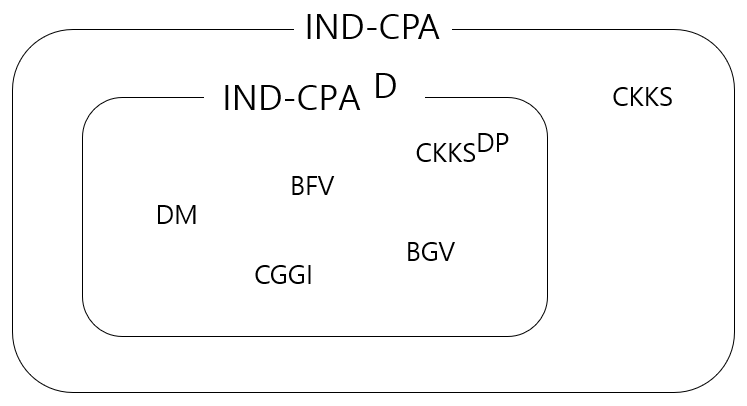
\includegraphics[width=0.7\linewidth]{diagram 1.png}
            \caption{The belief. }
        \end{figure}
    \end{frame}
    
    %%%%%
    % Li-Micciancio
    %%%%%    
    \begin{frame}{Prior Works}
    
    {\bf In the community}: 
    \begin{center}
        Exact FHEs, such as BFV/BGV,\\ and DM/CGGI schemes, are \indcpad secure!
    \end{center}\vspace{0.1cm}

        \begin{figure}[h]
            \centering
            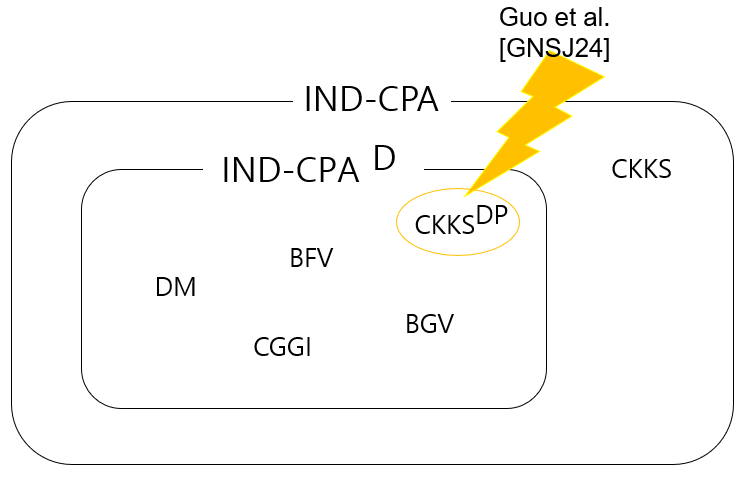
\includegraphics[width=0.7\linewidth]{diagram 2.png}
            \caption{Recent attack. }
        \end{figure}
    \end{frame}

    %%%%%
    % Really?
    %%%%%
    
    \begin{frame}{}
    \begin{center}
        {\Huge \bf Really?}
        % \vspace{1cm}\pause
        % {\large No, if the correctness is not sufficiently close to $1$.}
    \end{center} 
    \end{frame}

%%%%%%%%%%%%%%%%%
% Section 2: IND-CPA^D Insecurity
%%%%%%%%%%%%%%%%%
\section{\indcpad Security of FHEs:\\ {\normalsize Theoretical Results}}

    %%%%%
    % What if?
    %%%%%    
    \begin{frame}{What if?}

    What if \textcolor{blue}{$\dec_\sk(\enc_\pk(m)) \neq m$}, a.k.a. decryption fails?\vspace{0.2cm}\pause

    What if \textcolor{blue}{$\dec_\sk(\eval_\pk(C, \ct_1, \cdots, \ct_k))$}

    \hfill \textcolor{blue}{$\neq C(\dec_\sk(\ct_1), \dots, \dec_\sk(\ct_k))$},
    a.k.a. evaluation fails? \vspace{0.4cm}\pause

    $\Rightarrow$ $\cO_\enc$/$\cO_\eval$ will record $(m_0, m_1, \ct)$, which satisfies 
    \[
        \dec_\sk(\ct) \neq m_b.
    \]\pause

    Can we make a record satisfying $m_0 = m_1$, but $\dec_\sk(\ct) \neq m_0$?\vspace{0.3cm}\pause
        
    And, even, $\dec_\sk(\ct)$ depends on $b$? 
    \end{frame}

    \begin{frame}{}
    \begin{center}
        {\Large \bf Yes,\\\vspace{0.2cm} 
        with the failing probability!}
    \end{center} 
    \end{frame}
    
    %%%%%
    % Generic IND-CPA^D attack
    %%%%% 
	\begin{frame}{Generic \indcpad Attack}
	\begin{figure}[ht!]
    	\centering
    	\renewcommand{\arraystretch}{1}
    	{\small
    		\begin{tabular}{ccc}
                \underline{\bf $\cA$ (adversary)} & & \underline{\bf $\cC$ (challenger)}\\
                &&\\
    			&& $b \leftarrow \{0,1\}$\\
    			
    			& \hspace{-1.5cm}$\xxrightarrow{11111111111111111}{\cO_\enc (\texttt{T}, \texttt{F})}$ & $S[0] = (\texttt{T}, \texttt{F}, \ct_0)$\\
    			
    			& \hspace{-1.5cm}$\xxrightarrow{11111111111111111}{\cO_\enc (\texttt{F}, \texttt{F})}$ & $S[1] = (\texttt{F}, \texttt{F}, \ct_1)$\\

        		& \hspace{-1.5cm}$\xxrightarrow{11111111111111111}{\cO_\eval (\textsf{AND}(\cdot, \cdot), 0, 1)}$ & \pause $S[2] = (\texttt{T}\wedge\texttt{F} = \texttt{F}, \texttt{F} \wedge \texttt{F} = \texttt{F}, \ct_2)$\\
    			
    			& \hspace{-1.5cm}$\xxrightarrow{11111111111111111}{\cO_\dec (2)}$ & $m_{\textsf{res}} \leftarrow \dec_\sk(\ct_2)$\\
    			
    			& \hspace{-1.5cm}$\xxleftarrow{11111111111111111}{m_{\textsf{res}} }$ &\\
    			
    			$b' = \begin{cases}
    				0 & \text{if } m_{\textsf{res}} = \texttt{T} \enspace,\\
    				1 & \text{else}.
    			\end{cases}$ &&
    	  \end{tabular}
        }
    	\caption{Generic and passive \indcpad attack on binary FHE. \label{fig:indcpad_bin_1}}
    \end{figure}
	\end{frame}

    %%%%%
    % Generic IND-CPA^D attack (explanation)
    %%%%% 
	\begin{frame}{Generic \indcpad Attack}
	\begin{figure}[ht!]
    	\centering
    	\renewcommand{\arraystretch}{1}
    	{\tiny
    		\begin{tabular}{ccc}
                \underline{\bf $\cA$ (adversary)} & & \underline{\bf $\cC$ (challenger)}\\
    			&& $b \leftarrow \{0,1\}$\\
    			
                & \hspace{-1.5cm}$\xxrightarrow{11111111111111111}{\cO_\enc (\texttt{T}, \texttt{F}),~\cO_\enc (\texttt{F}, \texttt{F})}$ & $S[0] = (\texttt{T}, \texttt{F}, \ct_0)$, $S[1] = (\texttt{F}, \texttt{F}, \ct_1)$\\
    			
    			& \hspace{-1.5cm}$\xxrightarrow{11111111111111111}{\cO_\eval (\textsf{AND}(\cdot, \cdot), 0, 1)}$ & $S[2] = (\texttt{F}, \texttt{F}, \ct_2)$\\
    			
    			& \hspace{-1.5cm}$\xxrightarrow{11111111111111111}{\cO_\dec (2)}$ & $m_{\textsf{res}} \leftarrow \dec_\sk(\ct_2)$\\
    			
    			& \hspace{-1.5cm}$\xxleftarrow{11111111111111111}{m_{\textsf{res}} }$ &\\
    			
    			$b' = 0 \text{ if } m_{\textsf{res}} = \texttt{T} \enspace, \text{else } 1.$ &&
    	  \end{tabular}
        }
    \end{figure}
    {\small
    \begin{itemize}
        \item If no failure: $m_{\textsf{res}} = \texttt{F}$.\pause
        \item If $ct_0$ encryption fails\footnote{we ignore multiple failures, which gives quadratic terms}: $m_{\textsf{res}} = \texttt{F}$.\pause
        \item If $ct_1$ encryption fails (say, event $A$): $m_{\textsf{res}} = \texttt{T} \wedge \texttt{T} = \texttt{T}$ if $b=0$, and\\
        \hfill $\texttt{F} \wedge \texttt{T} = \texttt{F}$ if $b=1$.\pause
        \item If \eval fails: $m_{\textsf{res}} = \texttt{T}$.\pause
    \end{itemize}
    Thus, for $p = \Pr[A]$, the advantage of $\cA$ becomes 
        \begin{center}
        $\Pr[b=b']$ $\approx$ $(1-p) \cdot \Pr[b=b'~ |~ \neg\text{A}] + p \cdot \Pr[b=b' ~|~ \text{A}] = \frac{1}{2} + \frac{p}{2}$. 
        \end{center}
    }
	\end{frame}

    %%%%%
    % Generic IND-CPA^D attack (boosting)
    %%%%% 
	\begin{frame}{Boosting the \indcpad Attack}
 
    {\small
    \underline{\bf Boosting technique 1:} Repeating $N$ times?
    \begin{itemize}
        \item Advantage: $\frac{1}{2} + \frac{Np}{2}$,
        \item Cost: $2N$ \enc, $N$ \eval, $N$ \dec queries.
    \end{itemize}\pause\vspace{0.3cm}
    
    Instead, we can use a composed circuit: 
    \[
        C(x_0, \dots, x_{N}) = (x_0 \wedge x_1) \vee \dots \vee (x_0 \wedge x_N)
    \]
    \begin{itemize}
        \item Advantage: $\frac{1}{2} + \frac{Np}{2}$,
        \item Cost: $(N+1)$ \enc, but only 1 \eval, and 1 \dec queries!
    \end{itemize}
    }
	\end{frame}

    %%%%%
    % Generic IND-CPA^D attack (boosting)
    %%%%% 
	\begin{frame}{Boosting the \indcpad Attack}
 
    {
	\begin{figure}[ht!]
    	\centering
    	\renewcommand{\arraystretch}{1}
    	{\small
    		\begin{tabular}{ccc}
                \underline{\bf $\cA$ (adversary)} & & \underline{\bf $\cC$ (challenger)}\\
    			&& $b \leftarrow \{0,1\}$\\
    			
    			& \hspace{-2cm}$\xxrightarrow{11111111111111111}{\cO_\enc (\texttt{T}, \texttt{F})}$ & $S[0] = (\texttt{T}, \texttt{F}, \ct_0)$\\
    			
    			& \hspace{-2cm}$\xxrightarrow{11111111111111111}{\cO_\enc (\texttt{F}, \texttt{F}), \dots,~\cO_\enc (\texttt{F}, \texttt{F})}$ & $S[i] = (\texttt{F}, \texttt{F}, \ct_i)$ for $i=1,\dots,N$\\
    			
    			& \hspace{-2cm}$\xxrightarrow{11111111111111111}{\cO_\eval (C, 0, 1,\dots, N)}$ & $S[N+1] = (\texttt{F}, \texttt{F}, \ct_{N+1})$\\    			
    			
                & \hspace{-2cm}$\xxrightarrow{11111111111111111}{\cO_\dec (N+1)}$ & $m_{\textsf{res}} \leftarrow \dec_\sk(\ct_{N+1})$\\
    			
    			& \hspace{-2cm}$\xxleftarrow{11111111111111111}{m_{\textsf{res}} }$ &\\
    			
    			$b' = 0 \text{ if } m_{\textsf{res}} = \texttt{T} \enspace, \text{else } 1.$ &&
    	  \end{tabular}
        }
    \end{figure}

    \[
        \Pr[b=b'] \approx (1-p)^N \cdot \frac{1}{2}+ \left(1-(1-p)^N \right) \cdot 1 \approx \frac{1}{2} + \frac{Np}{2}
    \]
    }
	\end{frame}

    %%%%%
    % Generic IND-CPA^D attack (boosting)
    %%%%% 
	\begin{frame}{Boosting the \indcpad Attack}
 
    {
    \underline{\bf Boosting technique 2:} Replace $\ct_i$'s by the evaluated ciphertexts with \textcolor{blue}{higher (possibly the highest) probability $p^*$}($\gg p$): \pause\vspace{0.3cm}
    
    Advantage bumps up to $$\frac{1}{2} + \frac{Np^*}{2} ~ \left(\gg \frac{1}{2} + \frac{Np}{2}\right),$$
    with many \enc, but again, only 1 \eval, and 1 \dec queries\footnote{replace $C$ by $C \circ (id, C^*, \dots, C^*): \cC^{Nk+1} \rightarrow \cC$, where $C^*$ is the circuit with $k$ fresh ciphertexts as inputs and outputs a ciphertext having failing probability $p^*$}.
    }
	\end{frame}

    %%%%%
    % Generic IND-CPA^D attack (extension)
    %%%%% 
	\begin{frame}{Extending the \indcpad Attack}
 
    {
    \underline{\bf Extension:} The attack can be easily extended from binary FHEs to \textcolor{blue}{general integer FHEs}, as $\{0, 1\}$ can be embedded in any ring.\vspace{0.5cm}\pause
    
    E.g., use 0 and 1 instead of \texttt{F} and \texttt{T}; with \mult and \add instead of $\wedge$ and $\vee$, respectively. 
    }
	\end{frame}

    %%%%%
    % IND-CPA^D security conclusion
    %%%%% 
	\begin{frame}{Conclusion}
    Thus, the \textcolor{blue}{failing probability} of any \indcpad-secure FHE ciphertext \textcolor{blue}{should be negligible} along the whole homomorphic operations. \vspace{0.1cm}\pause
    \begin{center}
        HOWEVER,
    \end{center}
    
    \begin{itemize}
        \item {\bf DM/CGGI}
            \begin{itemize}
                \item {TFHE-rs}: $\mathsf{p}_\mathsf{fail} =2^{-40}$ (DEFAULT\_PARAMETERS set)\pause
                \item {{Concrete-Python}}: $\mathsf{p}_\mathsf{fail} =2^{-17}$ (default setting)\pause
                \item {Dahl et al.~\cite{cryptoeprint:2023/815}}: $\mathsf{p}_\mathsf{fail} =2^{-13.9}$
            \end{itemize}\vspace{0.3cm}\pause
        \item {\bf BFV/BGV}: Recent average-case approaches try to lower the correctness for more multiplicative levels:\pause
            \begin{itemize}
                \item {Murphy and Player~\cite{EPRINT:MurPla19a}}: $\mathsf{p}_\mathsf{fail} =0.001 \approx 2^{-10}$\pause
                \item {Biasioli et al.~\cite{cryptoeprint:2023/600}}: $\mathsf{p}_\mathsf{fail} =2^{-36} \sim 2^{-80}$
            \end{itemize}
    \end{itemize}\vspace{0.3cm}\pause
    \begin{center}
        \textcolor{blue}{\indcpad-secure? :(}
    \end{center}
	\end{frame}

%%%%%%%%%%%%%%%%%
% Section 3: KR^D Insecurity
%%%%%%%%%%%%%%%%%
\section{\krd Security of FHEs:\\ {\normalsize Practical Results}}

    % %%%%%
    % % BFV
    % %%%%%  
    % \begin{frame}{}
    % \begin{center}
    %     {\Huge \bf BFV}
    % \end{center} 
    % \end{frame}
    
    %%%%%
    % Average-case analysis
    %%%%%    
    \begin{frame}{Average-case Analysis on BFV}

    {\small
    RLWE ciphertext: $\ct = (\veca, \vecb = \veca\vecs + \Delta \vecm + \vece) \in \cR_Q^2$, $\operatorname{Var}(\vece) = \sigma^2$:
        \begin{figure}[ht!]
    	\centering
    	\begin{tikzpicture}[scale=0.8, every node/.style={scale=0.8}]
    		% Main rectangles
    		\draw (0,0) rectangle (6.5,1) {};
    		\node[anchor=east] at (0,0.5) {$\enc_\pk(0)=$};
    		
    		% Message rectangles
    		\draw [fill=gray!30](0,0) rectangle (1.5,1);
    		\node at (0.75,0.5) {$\vecm={\bf 0}$};
    		
    		% Error rectangles
    		\draw [fill=blue!20](5.5,0) rectangle (6.5,1);
    		\node at (6,0.5) {$\vece$};
    		
    		% Modulus
    		\draw[<->] (0,1.1) -- (1.5-0.01,1.1) node[pos=0.5, above] {$t$};
    		\draw[<->] (1.5+0.01,1.1) -- (6.5,1.1) node[pos=0.5, above] {$\Delta$};    
        \end{tikzpicture}
        \end{figure}
    $\Rightarrow \mathsf{p}_\mathsf{fail} = \operatorname{erfc}\left(t/\sqrt{2 \cdot \operatorname{Var}(e)}\right)$\vspace{0.5cm}\pause

    For $\ct + \ct'$, 
    \begin{itemize}
        \item Average-case analysis: $\operatorname{Var}(e+e') = 2\sigma^2$, assuming $\ct$ and $\ct'$ are independent.
        \item In the worst case ($\ct = \ct'$), $\operatorname{Var}(2e) = {4} \sigma^2$: $\mathsf{p}_\mathsf{fail}^\mathsf{worst} \gg \mathsf{p}_\mathsf{fail}^\mathsf{avg}$
    \end{itemize}\pause
    \begin{center}
        This gap makes the problem.
    \end{center}
    }
    \end{frame}

    %%%%%
    % KR^D Attack on BFV (figure)
    %%%%%    
    \begin{frame}{\krd Attack on BFV} 

    {\small
    {\bf Iterative addition attack\footnote{\scriptsize similar to the attack by Guo et al.~\cite{294637}, targeted Li and Micciancio's \indcpad-secure CKKS, implemented in OpenFHE~\cite{C:LMSS22}.}}: After $k$ additions, error $e$ blows up to $2^ke$, which will be decrypted to
    \[
        \round{({2^ke \bmod q})/{\Delta}} \approx e,
    \]
    if $2^k \approx \Delta$.\pause

    {\footnotesize
        \begin{figure}[ht!]
    	\centering
    	\begin{tikzpicture}[scale=0.8, every node/.style={scale=0.8}]
    		% Main rectangles
    		\draw (0,0) rectangle (6.5,1) {};
    		\node[anchor=east] at (0,0.5) {\small $\ct_0=$};
    		\draw (0,0-1.6) rectangle (6.5,1-1.6) {};
    		\node[anchor=east] at (0,0.5-1.6) {\small $\ct_{i+1}=$};
    		\draw (0,0-3.2) rectangle (6.5,1-3.2) {};
    		\node[anchor=east] at (0,0.5-3.2) {\small $\ct_k=$};
    		
    		% Message rectangles
    		\draw [fill=gray!30](0,0) rectangle (1.5,1);
    		\node at (0.75,0.5) {$\vecm={\bf 0}$};
    		\draw [fill=gray!30](0,0-1.6) rectangle (1.5,1-1.6);
    		\node at (0.75,0.5-1.6) {};
    		\draw [fill=gray!30](0,0-3.2) rectangle (1.5,1-3.2);
    		\node at (0.75,0.5-3.2) {};
    		
    		% Error rectangles
    		\draw [fill=blue!20](5.5,0) rectangle (6.5,1);
    		\node at (6,0.5) {$\vece$};
    		\draw [fill=blue!20](5.5-2.5,0-1.6) rectangle (6.5-2.5,1-1.6);
    		\node at (6-2.5,0.5-1.6) {$\vece$};
    		\draw [fill=blue!20](5.5-5,0-3.2) rectangle (6.5-5,1-3.2);
    		\node at (6-5,0.5-3.2) {$\vece$};
    		
    		% Modulus
    		\draw[<->] (0,1.1) -- (1.5-0.01,1.1) node[pos=0.5, above] {$t$};
    		\draw[<->] (1.5+0.01,1.1) -- (6.5,1.1) node[pos=0.5, above] {$\Delta$};
    		
    		% vdots
    		\node at (3.25, -0.17) {$\vdots$};
    		\node at (3.25, -0.17-1.6) {$\vdots$};
    
        \end{tikzpicture}
        \end{figure} 
    }\pause

    Note, average-case approach will allow this, since $\mathsf{p}_\mathsf{fail}^\mathsf{worst} \gg \mathsf{p}_\mathsf{fail}^\mathsf{avg}$. 
    }\vspace{0.1cm}
    \end{frame}

    %%%%%
    % KR^D Attack on BFV (result)
    %%%%%    
    \begin{frame}{\krd Attack on BFV (Result)} 

    {

    For a typical choice of OpenFHE 128-bit secure parameter set, \vspace{0.3cm}
    
    $N = 2^{12}$, $q=2^{60}$, $t = 2^{16}+1$, $\operatorname{std.dev}(e) = 2^{7.41}$, and $\Delta = \round{q/t} = 2^{44}-\varepsilon$, for some small $\varepsilon$, \vspace{0.3cm}
    
    we could experimentally reveal the exact error with $k=44$ iterations as
    \[
        \round{({2^{44}\vece \bmod 2^{60}})/(2^{44}-\varepsilon)} = \vece + \round{\varepsilon\vece / (2^{44}-\varepsilon)} = \vece,
    \]
    unless $\Vert\vece\Vert_\infty$ is too huge. 
    }
    \end{frame}

 
%%%%%%%%%%%%%%%%%
% Section 4: Threshold FHE Insecurity
%%%%%%%%%%%%%%%%%
\section{(In)security of Threshold FHE:\\ {\normalsize Theoretical Results}}

 %    %%%%%
 %    % (In)security of Threshold FHE
 %    %%%%% 
	% \begin{frame}{(In)security of Threshold FHE}

 %        Threshold FHE security: The attacker has access to partially decrypted results, so for\vspace{0.3cm}
	% 	\begin{itemize}
	% 		\item Threshold FHE scheme $\Pi$ (Setup, Enc, Eval, \textcolor{blue}{PDec}, \textcolor{blue}{FinDec}),
	% 		\item FHE scheme $\Pi^*$ (Setup, Enc, Eval, \text{Dec}), 
	% 	\end{itemize}
 %        where $\text{Dec}= \Pi.\text{FinDec}_{pk} \left(\left\{\Pi.\text{PDec}_{sk_i}(\cdot)\right\}_i\right)$, \vspace{0.3cm}
	% 	\[\bf
 %            \textbf{Threshold security of } \Pi ~\Rightarrow~ \indcpad \textbf{ security of } \Pi^*.
 %        \]
	% \end{frame}

    %%%%%
    % (In)security of Threshold FHE
    %%%%% 
	\begin{frame}{(In)security of Threshold FHE}

        Threshold FHE IND-security~\cite{cryptoeprint:2017/257}: The attacker has access to partially decrypted results if the underlying messages are the same,\vspace{0.4cm}
        
        \begin{figure}[h]
            \centering
            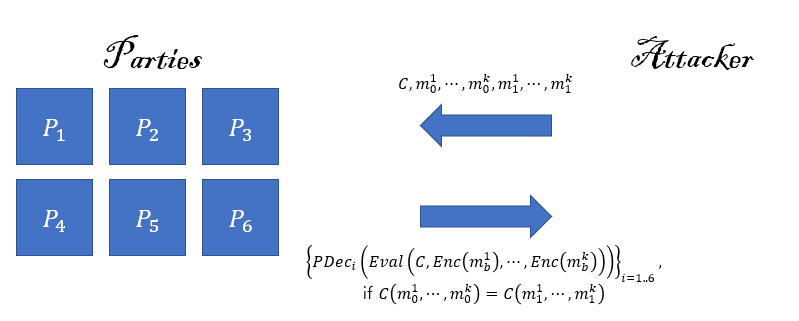
\includegraphics[width=\linewidth]{ThreshFHE.png}
            \caption{IND-security of Threshold FHE. }
        \end{figure}

        i.e., exactly the same as \indcpad!
	\end{frame}

    %%%%%
    % (In)security of Threshold FHE (reduction)
    %%%%% 
	\begin{frame}{(In)security of Threshold FHE}

        So, for
		\begin{itemize}
			\item Threshold FHE scheme $\Pi$ (Setup, Enc, Eval, \textcolor{blue}{PDec}, \textcolor{blue}{FinDec}),
			\item FHE scheme $\Pi^*$ (Setup, Enc, Eval, \text{Dec}), 
		\end{itemize}
        where $\Pi^*.\text{Dec} = \Pi.\text{FinDec}_{pk} \left(\left\{\Pi.\text{PDec}_{sk_i}(\cdot)\right\}_i\right)$, \vspace{0.3cm}
		\[\bf
            \textbf{Threshold {\normalfont IND-}security of } \Pi ~\Rightarrow~ \indcpad \textbf{ security of } \Pi^*.
        \]\vspace{0.3cm}\pause

        Note, the underlying FHE scheme of Noah's Ark~\cite{cryptoeprint:2023/815}, a CGGI-based Threshold FHE scheme, has $\mathsf{p}_\mathsf{fail} = 2^{-40}$ \textcolor{blue}{:(}
	\end{frame}
 
 %    %%%%%
 %    % A Hole in Noah's Ark
 %    %%%%% 
	% \begin{frame}{A Hole in Noah's Ark}

 %        Noah's Ark [WAHC:DDK+23]: CGGI-based Threshold FHE with ``Switch-and-Squash'' technique during PDec, which is
 %        \begin{center}
 %        essentially ``ModSwitch'' to larger modulus $2N$,
 %        \end{center}

 %        of failure probability $\mathsf{p}_\mathsf{fail} = 2^{-72.8}$ to $2^{-85.1}$.\vspace{0.3cm}\pause

 %        Note, the underlying FHE scheme already has $\mathsf{p}_\mathsf{fail} = 2^{-40}$. 
	% \end{frame}
 
%%%%%%%%%%%%%%%%%
% Summary
%%%%%%%%%%%%%%%%%

 \section{Summary}
    %%%%%
    % Summary
    %%%%%    
    \begin{frame}{Summary}
    \small
    Theoretical results: 
    \begin{itemize}
        \item Exact FHE schemes are also \indcpad-insecure \textcolor{blue}{unless} it has a negligible failure probability\footnote{during the whole homomorphic operations.}.\pause
        \item Threshold FHE schemes are IND-insecure \textcolor{blue}{unless} the underlying FHE schemes are \indcpad-secure. 
    \end{itemize}\vspace{0.3cm}\pause
    
    Practical results: \krd attacks on
        \begin{itemize}
            \item BFV\pause
            \item CGGI (not included)
            \item CGGI-based Threshold FHE scheme, {Noah's Ark}\footnote{even if the underlying FHE scheme is perfectly correct!} (not included)
        \end{itemize}\vspace{0.5cm}
    \end{frame}
    
    %%%%%
    % Summary (Diagram)
    %%%%%    
    \begin{frame}{Summary}

        \begin{figure}[h]
            \centering
            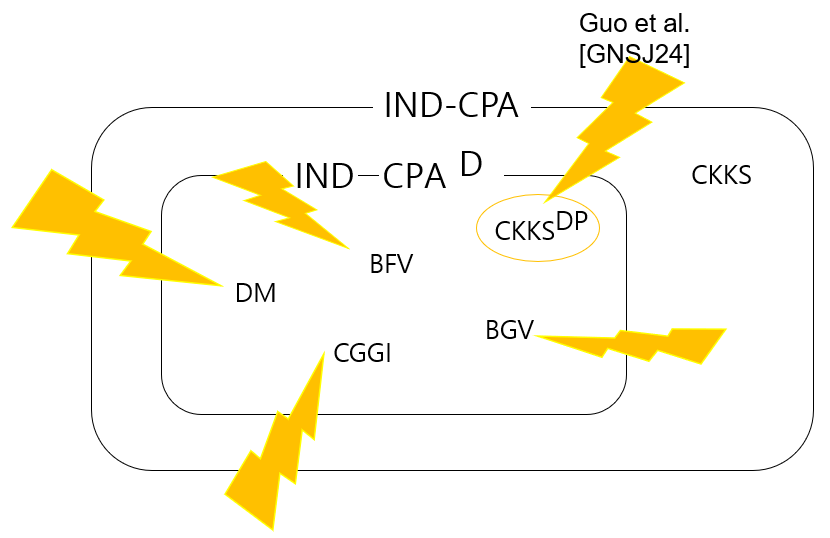
\includegraphics[width=0.7\linewidth]{diagram 3.png}
            \caption{Our attack. }
        \end{figure}
    \end{frame}
    
    %%%%%
    % Thank You
    %%%%%    
    \begin{frame}{}
    \begin{center}
        {\Huge\bf Thank You!}
    \end{center}
    \end{frame}
    
    %%%%%
    % Bibliography
    %%%%%    
    \setbeamertemplate{bibliography item}{\insertbiblabel}
    \begin{frame}[t, allowframebreaks, noframenumbering, plain]{References}
    
    \bibliographystyle{alpha}
    \bibliography{20240104_reduced/cryptobib/abbrev3,20240104_full_version/cryptobib/crypto,ref}
    
    \end{frame}

    %%%%%%%%%%%%%%%%%%%%%%%%%%%%%%%%%%%%%%%
    %%%%%%%%%%%%%%%%%%%%%%%%%%%%%%%%%%%%%%%

    %%%%%
    % CGGI
    %%%%%  
    \begin{frame}{}
    \begin{center}
        {\Huge \bf CGGI}
    \end{center} 
    \end{frame}   
    
    %%%%%
    % CGGI Modulus Switch
    %%%%%
	\begin{frame}{CGGI Modulus Switch}
		\begin{center}
			\begin{tikzpicture}[node distance=3.5cm,>=latex']
				
				\tikzstyle{block} = [rectangle, draw, text centered, text width=3cm, minimum height=1.5cm, node distance=4cm, rounded corners]
				\tikzstyle{arrow} = [->,>=latex']
				
				\node [block, fill=blue!30] (lwe) {$\mathsf{LWE}_{q \approx 2^{32}}$\\ Var$(\vece) = \sigma^2$};
				\node [block, right of=lwe, fill=orange!30, rounded corners] (bootstrap) {Modulus\\ Switch};
				\node [block, right of=bootstrap, fill=blue!30] (lwebr) {\small $\mathsf{LWE}_{2 N \approx 2^{10}}$\\Var$(\vece + \vece_{MS}) = \sigma^2 + \sigma_{MS}^2$};
				
				\draw [arrow] (lwe) -- (bootstrap);
				\draw [arrow] (bootstrap) -- (lwebr);
				
			\end{tikzpicture}
		\end{center}
        \[
            \ct \mapsto \round{\ct\cdot 2N / q}
        \]
  
		Modulus Switching error: $\vece_{MS} := \langle \vec{e}_{MS}, \sk \rangle$, $\operatorname{Var}(\vec{e}_{MS}) = \sigma_{MS}^2 \gtrsim \sigma^2$. \vspace{0.3cm}\pause

        Modulus Switching failure: $\vece + \langle \vec{e}_{MS}, \sk \rangle > t$, for a threshold $t$, with probability 
        \[
        \mathsf{p}_\mathsf{fail} = \operatorname{erfc}\left(t/{\sqrt{2 (\sigma^2 + \sigma_{MS}^2)} }\right) \approx 2^{-40}.
        \]
	\end{frame}

    %%%%%
    % CGGI KR^D attack
    %%%%%
	\begin{frame}{$KR^D$ attack on CGGI}

    {\small \vspace{-0.1cm}
		\begin{block}{Lemma.}\vspace{0.1cm}
			Let~$Y_i = \langle \vec{e}_{MS}, \sk \rangle - e_{MS, i} \cdot \sk_i$.
			The probability density function~$f$ of~$e_{MS,i}$ conditioned on the event $\langle \vec{e}_{MS}, \sk \rangle + e > t$ (i.e. failure) satisfies, for all~$x \in [-1/2,1/2]$: 
			\[
			f(x) = \left\{
			\begin{array}{ll}
				\frac{\Pr[x + Y_i + e > t]}{\Pr[ \langle \vec{e}_{MS}, \sk \rangle + e > t]}& \text{if } \sk_i=\textcolor{blue}{1}, \\
				1& \text{if } \sk_i = \textcolor{orange}{0}.
			\end{array}\right.\]
		\end{block}\vspace{-0.3cm}\pause
    }

        \begin{figure}[h]
            \centering
            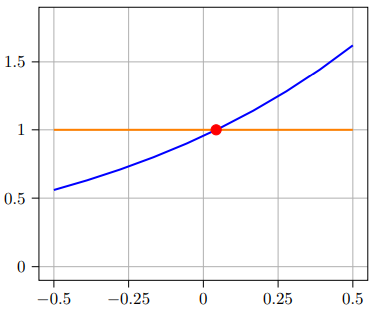
\includegraphics[width=0.4\linewidth]{slope.png}
            \caption{Distribution of $e_{MS, i}$ conditioned on decryption failures (pdf $f$). }
        \end{figure}
	\end{frame}
 
	\begin{frame}{Experimental results}
		\begin{figure}
			\centering
			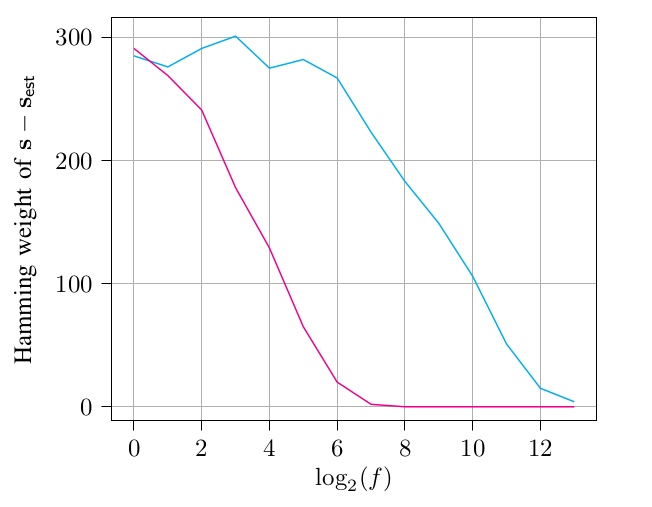
\includegraphics[width=0.7\linewidth]{exp}
			\caption{Performance of the attack (score: $\Vert \vecs - \vecs_\mathsf{est} \Vert_1$) with ``$f$'' failing ciphertexts. Experimental result for a \textcolor{cyan}{custom parameter} set and a simulated result for \textcolor{magenta}{TFHE-rs DEFAULT\_PARAMETERS} set is given.}
			\label{fig:tkrd}
		\end{figure}
	\end{frame}

    %%%%%
    % CGGI
    %%%%%  
    \begin{frame}{}
    \begin{center}
        {\Large \bf Noah's Ark, a Threshold FHE}
    \end{center} 
    \end{frame}   
    
    %%%%%
    % A Hole in Noah's Ark
    %%%%% 
	\begin{frame}{A Hole in Noah's Ark}

        Noah's Ark~\cite{cryptoeprint:2023/815}: CGGI-based Threshold FHE with ``Switch-and-Squash'' technique during PDec, which is
        \begin{center}
        essentially ``ModSwitch'' to larger modulus $2N$,
        \end{center}

        of failure probability $\mathsf{p}_\mathsf{fail} = 2^{-72.8}$ to $2^{-85.1}$.\vspace{0.3cm}\pause

        Thus, even if the underlying FHE scheme is perfectly correct, the ``Switch-and-Squash'' technique makes it insecure.
	\end{frame}
    
    %%%%%
    % Future Works?
    %%%%% 
	\begin{frame}{Future Works?}

        \begin{itemize}
            \item Security of Threshold/Multi-Party FHE
            \item Circuit privacy and \indcpad security
            \item Securing Threshold/Multi-Party FHE with sanitization
        \end{itemize}
	\end{frame}
\end{document}
